
\documentclass[a4paper,12pt,table]{scrreprt}
\usepackage{graphicx} % obrazky
\graphicspath{{images/}} % cesta k obrazkum
\usepackage{pdfpages} % include na pdf zadani
\usepackage{verbatim} % komentare
\usepackage[section]{placeins} % obrazky pod kapitolama
\makeatletter
\usepackage[font=small,labelfont=bf]{caption} %captiony
\usepackage{amsmath} % matematika bez cisel
\usepackage{chngpage}
\usepackage{setspace}

%ROZTAZENI PISMA---------
\tolerance=1
\emergencystretch=\maxdimen
\hyphenpenalty=10000
\hbadness=10000

\usepackage[czech]{babel} % localize labels to czech (Obsah, Kapitola, Literatura atp.)
%PDF SETUP--------- DEPRECATED !
\usepackage[hidelinks]{hyperref} %odkazy v  pdf jsou klikací s barevnými rámečky
\hypersetup{   % some PDF metadata
	pdftitle={Návrh a realizace software pro analýzu biomedicínských dat},%   
	pdfauthor={Lukáš Sulík},%  
	pdfsubject={},%   
	pdfkeywords={}%                             
}

%BIBLIOGRAFIE---------
\usepackage[backend=bibtex,sorting=none,bibstyle=ieee]{biblatex}
\addbibresource{bibliography.bib}

%TABLE---------
%\setlength{\arrayrulewidth}{1px}

%LAYOUT---------
\renewcommand{\baselinestretch}{1.5} %radkovani s
\setlength{\parindent}{4em} % odsazeni odstavcu
\usepackage[automark,headsepline]{scrlayer-scrpage}
\clearpairofpagestyles
\rofoot[\pagemark]{\pagemark}
\rohead{\rightmark}
\pagestyle{scrheadings}


%FONT---------
\usepackage{mathptmx} %matematika ala times 
\usepackage{tgtermes} %české písmo times 
\renewcommand{\sfdefault}{qhv} % české bezšerivové písmo helvetika
\renewcommand{\ttdefault}{qcr}%český curier
\usepackage{cmap}%kvůli prohledávatelnosti pdf souboru
\usepackage[T1]{fontenc}
\usepackage[utf8]{inputenc}

%GLOSSARY---------
\usepackage[toc]{glossaries}

\makeglossaries

\begin{document}
	\cleardoublepage{}~\thispagestyle{empty}\begin{center}\pagenumbering{roman}
	
	\textsf{\Large Univerzita Hradec Králové}
	
	\vspace{0.5em}
	\textsf{\Large Fakulta informatiky a managementu}
	
	\vspace*{1em}
	\textsf{\Large Katedra informatiky a kvantitativních metod }
	
	\vspace{15mm}
	
\includegraphics[width=0.5\textwidth]{images/uhk}
	
	\vspace{10mm}
	\textsf{\LARGE DIPLOMOVÁ PRÁCE}
	
	\vspace{10mm}
	\textsf{\LARGE Návrh a realizace software pro analýzu biomedicínských dat}
	
	\vspace{10mm}
\end{center} 

\vspace{10mm}
\begin{description}
	\item [{{\large Autor:}}] \noindent \textsf{\large Lukáš Sulík}
	\item [{{\large Studijní obor:}}] \noindent \textsf{\large AI2}
	\item [{{\large Vedoucí práce:}}] \noindent \textsf{\large doc. Ing. Ondřej Krejcar, Ph.D.}
\end{description}
\vfill
\hspace{2.5em}\textsf{\large Hradec Králové} \hfill \textsf{\large 2015}
\clearpage{}

%{\small \thispagestyle{plain}\addcontentsline{toc}{chapter}{Abstrakt} }{\small \par}

\newpage{}\thispagestyle{plain}

{\small \setcounter{page}{2} % nastavení číslování stránek
	\ }{\small \par}

\noindent {\small \vfill{}
	% set next text to bottom
	~}{\small \par}

\subsubsection*{Prohlášení}

\noindent Prohlašuji, že jsem diplomovou práci zpracoval samostatně a s použitím uvedené literatury.

\bigskip{}
\noindent V Hradci Králové dne \today\hspace{10em} Podpis:

\clearpage{}

\newpage{}\thispagestyle{plain}

{\small %\setcounter{page}{3} % nastavení číslování stránek
	\ }{\small \par}

\noindent {\small \vfill{}
	% set next text to bottom
	~}{\small \par}

\subsubsection*{Poděkování}

\noindent Rád bych poděkoval vedoucímu diplomové práce doc. Ing. Ondřeji Krejcarovi, Ph.D. za ochotu a úsilí vést tuto práci. Dr. Orcanovi Alparovi za konzultace ohledně vyvíjených algoritmů. A v neposlední řadě své rodině a přátelům, kteří mě při studiu podporovali.

\clearpage{}

\newpage{}\thispagestyle{plain}

\subsubsection*{Anotace}

Práce v teoretické části představuje kapslovou endoskopii a její využití ve zdravotnictví a zároveň základy počítačového vidění, jeho úskalí a přednosti. A dále představuje i několik základních algoritmů, které se v práci používají a průzkum trhu, jenž analyzuje aktuální stav technologií. Praktická část je založena na vývoji nového programu pro kapslovou endoskopii a základních algoritmů pro detekci krvácení v tenkém střevě. Výsledkem práce je software na platformě Java, využívající knihovnu OpenCV, který dokáže detekovat krvácení v zažívacím traktu.

\subsubsection*{Annotation}

Theoretical part of the thesis presents capsule endoscopy and its use in healthcare and basics of computer vision, its pitfalls and advantages. Along with that, it is presented several fundamental algorithms that are used in the thesis and market research, which analyzes the current state of the art. Practical part is based on the development of a new program for capsule endoscopy and basic algorithms for detecting bleeding in the small intestine. The result is software based on the Java platform, using the OpenCV library and it can detect bleeding in the digestive tract.

\cleardoublepage{}

{\small %%%   place for the signature
	%%%                                         *********
}{\small \par}

\cleardoublepage{}\thispagestyle{empty}
\tableofcontents{}
	\pagenumbering{arabic}
	\chapter{Úvod}
S nárůstem moderních technologií se rozvijí také lékařské odvětví. Dnes je již téměř vše řízené alespoň částečně pomocí počítačů a je snaha co nejvíce úkonů zautomatizovat, aby se lékaři mohli soustředit pouze na věci, které vyžadují jejich odborné znalosti a zkušenosti.

Kapslová endoskopie se zabývá analýzou tenkého střeva. To je nejobtížnější část střeva k prozkoumání, z důvodu vzdálenosti od úst a řitního otvoru a jeho komplikovaného tvaru, který může obsahovat různé smyčky. Konvenční endoskopické techniky např. enteroskopie nebo kolonoskopie jsou limitovány délkou tenkého střeva (3.35–7.85 m)\cite{randomized}, a proto je potřeba získávat data způsobem, který přinesla právě kapslová endoskopie.

Získaná data je nutné vyhodnotit a to může provést osoba s potřebnými znalosti k tomu určená, což přináší hned několik úskalí. Vzhledem k množství vyšetření a délky záznamu spotřebovává spoustu času projetí všech záznamů a určení diagnózy. To má za následek větší časovou náročnost na odborníky a také, pokud má pacient nějaký akutní problém, chvíli potrvá, než se podaří odhalit ze záznamů jeho příčinu.

Z těchto důvodů je často lékařské odvětví propojováno s rozhodovacími a vyhodnocovacími systémy, které zpracovávají nepřeberné množství dat a usnadňují tím lékařům práci. Specializované biomedicínské programy pak dokáží rychle identifikovat zdroj choroby a zkrátí tím čas, který by byl potřebný k projetí všech dat. V případě, že program nalezne nějakou anomálii, lékař hned objeví zdroj problému a může stanovit diagnózu podstatně rychleji. Samozřejmě, že tyto systémy nemohou plně nahradit znalosti a zkušenosti odborníků, z právního hlediska tak činit ani nesmějí, mohou však minimálně usnadnit jejich práci.

\section{Cíle práce}
Cílem této práce je navrhnout systém, který by dokázal zpracovávat data z kapslové endoskopie. Měl by být konkurenceschopný mezi aktuálními systémy na trhu.

Konkrétním úkolem systému pro tuto diplomovou práci je z dodaných dat analyzovat, zdali se v nich nachází stopy po krvácení. Kromě detekce krve systém musí být připraven i na další možné rozšíření v podobě nových detekčních algoritmů i pro jiné nemoci, které by se mohly implementovat později, pokud se systém ověří. Algoritmy pro detekci krve je nutné zaměřit na co největší rozsah detekce, aby byla téměř 100\% jistota, že bude krev nalezena.

Systém bude ověřen na vzorcích dat dodaných Fakultní nemocnicí Hradec Králové, s kterou bude posuzována i funkčnost a využitelnost daného řešení.

Aktuální návrh systému počítá s implementací GUI v podobě desktopové aplikace, jež bude spustitelná nezávisle na zvolené platformě, prioritně na Microsoft Windows. Systém však musí být schopný snadné rozšiřitelnosti v podobě implementace jiného GUI, např. webové aplikace.
\section{Kapslová endoskopie}
Kapslová endoskopie spočívá v malé kapsli o velikosti větší pilulky, jež má vlastní zdroj světla, kameru, anténu a zdroj energie viz obrázek \ref{fig:capsule}. Kamera snímá obraz ze střeva a posílá ho bezdrátově do přijímače umístěného mimo pacientovo tělo. V současné době existuje několik výrobců, jejichž specifikace kapsle se může mírně lišit. Jsou jimi např.:
\begin{itemize}
	\item Olympus EC-S10 – 11x26 mm, výdrž až 12 hodin.\cite{endocapsule}
	\item IntroMedic MicroCam – 11x24mm, výdrž 11+ hodin.\cite{intromedic}
	\item GivenImaging PillCam SB3 – 11x26mm, výdrž 8+ hodin.\cite{pillcam}
\end{itemize}

\begin{figure}[h]
	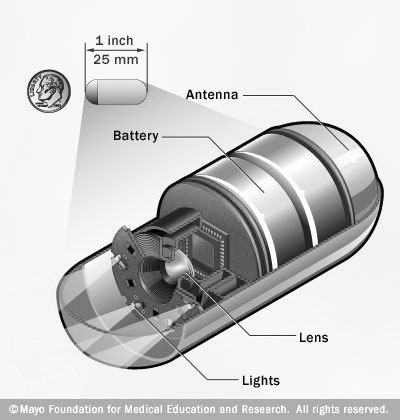
\includegraphics[]{capsule}
	\centering
	\caption{Kapsule \cite{capsule}\label{fig:capsule}}
\end{figure}

Ve většině případů je zapotřebí okolo osmi hodin \cite{diagnosing} pro průchod celým zažívacím traktem. Po dokončení celého procesu je kamera vyloučena z pacientova těla přirozenou cestou a již se nedá znovu použít. Vyšetření se provádí za účelem zjištění následujících nemocí (volně přeloženo z \cite{capsule}):

\begin{itemize}
\item Krvácení v zažívacím traktu - kapslová endoskopie může pomoci při určení příčiny krvácení.
\item Zánětlivé onemocnění střev - kapslová endoskopie může odhalit místa zánětu v tenkém střevě a tak pomoci diagnostikovat Crohnovu nemoc a další zánětlivá onemocnění.
\item Rakovina - kapslová endoskopie může identifikovat nádory v tenkém střevě, které by jinak byly těžko identifikovatelné. Kapslová endoskopie je občas prováděna se spojením s magnetickou rezonancí, protože magnetická rezonance může odhalit nádory ve stěně tenkého střeva.
\item Celiakie - některé malé studie tvrdí, že kapslová endoskopie může detekovat střevní změny spojené s celiakií - alergickou reakci po požití lepku - a může detekovat komplikace.
\item Polypy - lidé, kteří mají vrozenou polypózu, která může způsobovat polypy v tenkém střevě např. Peutz-Jeghersův syndrom, tak mohou využívat kapslovou endoskopii pro zobrazení polypů.
\end{itemize}


	\chapter{Počítačové vidění v endoskopii}
\section{Úvod do počítačového vidění}
Počítačové vidění (dále jen \gls{glos:CV}) je obor výpočetní techniky jehož počátky sahají do 60. let minulého století. Tomuto oboru se v posledních letech dostalo velkého rozmachu. Na trh se dostává stále více zařízení schopných snímat obrazová data,vzrůstá jejich kvalita a cena klesá. Ač \gls{glos:CV} není vyloženě určeno nějakou definicí,dalo by se říci, že \gls{glos:CV} je strojové porozumění obrazu, který se získává ze snímacích zařízení (např. různé fotoaparáty či kamery). V podstatě by se dalo srovnat s viděním biologickým s tím rozdílem, že u většiny vícebuněčných organismů jde o naprosto přirozenou a běžnou věc.\cite{learning}\cite{image} \gls{glos:CV} najde zastoupení v celé řadě odvětví např.

\begin{itemize}
	\item Automatizovaný průmysl - čidla pro kontrolu vadností výrobku, ovládání robotů, řízení logistických procesů, ...
	\item Medicína - zpracování obrazových dat z mikroskopů, ultrazvuku, endoskopii, RTG, ... \gls{glos:CV} zkvalitňuje diagnostické nástroje a je již standardní součástí diagnostických procesů.
	\item Armáda - automaticky naváděné rakety, detekce pohybu vojáků, bezpilotní stroje (letadla, ponorky, ...)
	\item Zábavní průmysl - interakce mezi strojem a člověkem. Např. ovládání počítačové hry gesty.
	\item Rozšířená realita - v kombinaci s počítačovou grafikou je základním prvkem v rozšířené realitě. Např. Microsoft hololens.
	\item A mnoho dalších.
\end{itemize}

Oproti biologickému vidění se jedná z pohledu zpracování o velice komplikovanou věc. Počítač přijímá pouze číselné hodnoty jako obrazová data. Proto je pro lidský druh snadné identifikovat např. auto na obrázku \ref{fig:car}, ale pro stroj je nutné definovat auto, jako složitý matematický model. \gls{glos:CV} také naráží na problémy, které vznikají při sběru dat. Jsou jimi: (volně přeloženo z \cite{image}).
\begin{itemize}
	\item 3D > 2D - ztráta prostorové informace. Obraz z reálného světa je uložen jako 2D. Díky modelu dírkové komory\footnote{z anglického pinhole model} jsou malé objekty blízké kameře stejné jako velké vzdálené objekty. Lidé jsou schopni tyto objekty rozeznat, pokud je v obraze nějaký objekt, u kterého znají jeho velikost, např. krabička od sirek.
	\item Interpretace - porozumění obsahu scény. Lidský mozek vyhodnocuje obraz pomocí svých znalostí a zkušeností. A proto je schopný vyhodnocovat nové problémy, které předtím neznal. Zatímco takováto schopnost strojů je velice omezená a její zdokonalení je klíčem k inteligentním systémům. Počítač je schopen analyzovat obraz pomocí matematické logiky, sémantiky a teorií formálních jazyků. Pokud je znám algoritmus pro řešení určitého problému, je možno analyzovat obraz, např. řeka v satelitním obrazu.
	\item Šum - je přítomný v každém měření v reálném světě.
	\item Příliš mnoho dat - Obrázky a videa jsou obrovské. Stránka A4, 300 dpi, 8 bit per pixel = 8,5 MB. Neprokládané video 512 x 768, RGB (24 bit) = 225 MB/s. Je proto tak těžké dosáhnout složité analýzy v reálném čase.
	\item Měřený jas - je dán složitým fyzikálním postupem vytváření obrazu. Zář závisí na ozáření (typ světelných zdrojů, jejich poloha a intenzita),
	poloze pozorovatele, lokální geometrii povrchu a odrazivosti povrchu.
	Obrácená úloha je špatně podmíněna.
	\item Lokální okno versus potřeba globálního pohledu - počítač vidí svět pouze z pohledu klíčové dírky bez celkového kontextu. Je proto těžké určit kontext obrazu, pokud je dostupná jen jeho část. Lidský mozek je schopný si domyslet potřebné informace pro určení, pokud je zná.
\end{itemize}

\begin{figure}[h]
	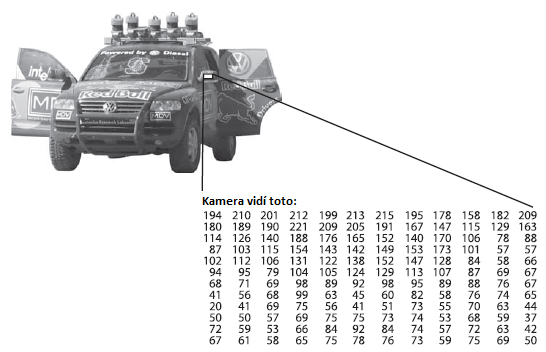
\includegraphics[]{car}
	\centering
	\caption{Auto přeloženo z\cite{learning}\label{fig:car}}
\end{figure} 


Zpracování obrazu počítačem se dá rozdělit na několik úrovní a výsledkem je řetězec, kde se postupuje od nejnižší po nejvyšší úroveň. Na nejnižší úrovni se zpracovávají surová data, která jdou přímo ze snímacích senzorů. Poté, co je obraz z nejnižší úrovně zpracován, používají se metody pro odstranění šumu, detekce hran, barevná filtrace či různá komprese obrazu. Těmito úpravami vznikne obraz, ze kterého lze již přejít k vyšší úrovni zpracování a tím je porozumění daného obrazu. Na této úrovni se dají aplikovat poznatky z umělé inteligence (např. neuronové sítě) nebo matematické definování objektů pro určení výsledného významu obrazu. Vyšší úroveň zpracování je nejtěžší věc na \gls{glos:CV}, často není ani možné dosáhnout požadovaného výsledku a vše se musí zjednodušovat, aby se dosáhlo alespoň výsledku částečného. \cite{learning}\cite{image}

\section{Algoritmy počítačového vidění}
V biomedicíně se používá většina známých algoritmů z počítačového vidění. Jelikož je jich velké množství, jsou pro charakter této práce popsány pouze ty, které se pak používají v praktickém řešení konkrétního problému této práce. Všechny tyto základní známé algoritmy jsou implementovány v knihovnách či programech pro počítačové vidění, např. OpenCV nebo Matlab.

\subsection{Konverze barevných formátů}
Obrazová data, s nimiž se v počítačovém vidění pracuje, jsou reprezentována různými grafickými schématy. V této práci se vyskytuje převážně schéma RGB, ve kterém jsou uložena data. Dále se pracuje s HSV a GrayScale.

\begin{itemize}
	\item RGB formát je aditivní míchání červené, zelené a modré barvy. Každý bod na obrázku je udáván jako vektor tří elementů, tedy intenzitou tří základních barev.\cite{image}
	\item HSV formát se skládá ze tří složek: barevný tón(hue), sytost(saturation) a hodnota jasu neboli množství bílého světla (value). Je velice blízký lidskému vnímání barvy a to zejména tónu a sytosti. Tento formát se hojně používá při algoritmech pracujících s obrazem.\cite{image}
	\item Grayscale vyjadřuje data pouze v odstínech šedi. Každá hodnota je definována na stupnici šedi a výsledný obraz je tak černo-bílý.
\end{itemize}

Převody mezi těmito formáty nejsou triviální záležitostí a jsou pro ně definovány složité vzorce. Na obrázku \ref{fig:colorspace} lze vidět ukázku barevných schémat. 

\begin{figure}[h]
	
\includegraphics[scale=0.5]{colorspace}
	\centering
	\caption{Barevná schémata zleva: RGB, HSV a GrayScale}\label{fig:colorspace}
\end{figure}

\subsection{Práhování}
Práhování\footnote{Z anglického threshold} je nejjednodušší z metod segmentace obrazu. Metoda spočívá v definování hranice hodnot, která bude sloužit pro rozhodnutí, bude-li daný bod v obraze  akceptován či nikoliv. To, co se bude dít s akceptovaným a neakceptovaným bodem, záleží na konkrétní metodě. Mezi základní patří:\cite{opencv}

\begin{itemize}
	\item Binární - Akceptovaný bod je nastaven na 1, ostatní na 0.
	\item Osekání - Akceptovaný bod je ponechán. Ostatní jsou zahozeny.
	\item Do nuly - Pokud je bod menší než daná hranice, tak je nastaven na 0. Ostatní jsou ponechány.
\end{itemize}

\begin{figure}[h]
	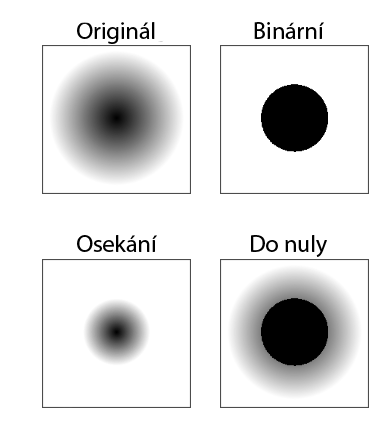
\includegraphics[scale=0.5]{threshold}
	\centering
	\caption{Metody práhování převzato z \cite{opencv}}\label{fig:threshold}
\end{figure}

Mezi složitější metody práhování patří adaptivní práhování, kde práh není stejný po celou dobu běhu algoritmu, ale je určován dynamicky. Dá se tím docílit lepších výsledků  při různých světelných podmínkách. Hodnota práhu může být vypočítána průměrem okolních hodnot nebo pomocí váženého součtu okolních bodů, kde váhy jsou Gaussovo okno.\cite{opencv}

\subsection{Morfologické operace}
Morfologické operace představují zpracování snímků založených na tvarech. Ve struktuře se generuje vstupní obraz na výstupní obraz. Uplatnění nachází především v oblastech spojování nesourodých prvků v obraze, hledání intenzity hrbolů nebo dírek v obraze či změny tvaru a velikosti geometrických objektů. Mezi základní morfologické operace patří eroze a dilatace.\cite{eroding}

Dilatace se skládá z obrazu (A), který v sobě skrývá jádro (B) určitého tvaru, nejčastěji čtverce nebo kruhu. Jádro má definován tzv. kotevní bod, který představuje střed jádra. Toto jádro je skenováno přes obraz. Počítáním maximální hodnoty pixelu překrytého jádra B a obrazového pixelu v bodě poloze kotvy způsobí světlé oblasti v obraze.  Dilataci můžeme vyjádřit jako sjednocení posunutých bodových množin. Uplatní se především v případech nutnosti zaplnění malých děr, úzkých zálivů, zvětšení objektů či použití jako stavební kámen složitějších operací. \cite{eroding}

Eroze je považována za sestru dilatace. Umožňuje spočítání lokálního minima přes oblast jádra. Jádro B je skenováno přes obraz a výpočtem minimální hodnoty vrátí obrazový pixel kotevního bodu.\cite{eroding}

\begin{figure}[h]
	
\includegraphics[scale=0.5]{morfoperace}
	\centering
	\caption{Morfologické operace převzato z \cite{eroding}}\label{fig:morfoperace}
\end{figure}

\subsection{Vyhlazování obrazu}
Vyhlazování obrazu, mnohdy také nazývané jako rozmazávání, je často používaná a jednoduchá operace při zpracování obrazu. Díky této operaci dosáhneme vyhlazení obrazu, například za účelem snížení šumu. Pro vyhlazování jsou používány nízkoprůchodové, nejčastěji lineární filtry, jako konvoluční matice. Tím se odstraní vysokofrekvenční obsah, např. hrany nebo šum.\cite{opencv:} Nejpoužívanější filtry jsou:

\begin{itemize}
	\item Normalizovaný filtr - pro každý pixel je spočítán průměr z jeho samého a okolí. Velikost okolí závisí na zvolené velikosti konvoluční matice. Filtr se používá pro odstranění vysokých frekvencí v obraze.\cite{opencv:}
	\item Gaussův filtr - konvoluční matice je vypočtena pomocí 2D Gaussovy rovnice. Jelikož by byl výsledek nekonečný, musí se specifikovat velikost matice a do ní se pak spočtou váhy Gaussova vrcholu. Filtr se používá pro odstranění šumu a vyhlazení obrazu.\cite{opencv:}
	\item Medián filtr - algoritmus vezme všechny pixely z konvoluční matice a určí jejich medián. Jím je pak nahrazen zpracovávaný pixel. Filtr se využívá pro odstranění "sůl a pepř" šumu.\cite{opencv:}
	\item Bilaterální filtr - je podobný Gaussovu filtru, ten bere v potaz všechny body, které se nachází v konvoluční matici, ale již neřeší jejich intenzitu. Bilaterální filtr proto používá ještě další funkci a zahrnuje pouze ty body v matici, jejichž intensita je podobná, jako právě zpracovávaného. To má za následek, že filtr vyhlazuje obraz, ale zachovává hrany. \cite{opencv:}
\end{itemize}

\begin{figure}[h]
	
\includegraphics[scale=0.7]{filtry}
	\centering
	\caption{Ukázka filtrů z průběhu práce}\label{fig:filtry}
\end{figure}

\subsection{Detektory hran}
Detektory hran jsou velmi důležité pro algoritmy počítačového vidění. Neurofyziologický a psychofyzický výzkum ukazuje, že pro zrakové vnímání vyšších organismů jsou důležitá místa v obraze, kde se náhle mění hodnota jasu. Místa jež odpovídají významným hranám, nesou více informací než jiná místa v obraze. Je zde proto možné značně zredukovat množství dat, aniž by došlo k významné redukci informací o obraze.\cite{image}

Mezi nejpoužívanější hranové detektory patří Cannyho hranový detektor, který také završil hledání po ideálním detektoru hran. Byl vymyšlen Johnem F. Cannym v roce 1986 a míří k uspokojení tří kriterií:
\begin{itemize}
	\item Minimální počet chyb - algoritmus musí detekovat všechny důležité hrany a neměly by být detekovány žádné falešné výsledky.
	\item Přesnost - rozdíl polohy skutečné a detekované hrany musí být minimální.
	\item Jednoznačnost - pouze jeden výsledek pro jednu hranu. Toto je částečně pokryto bodem jedna - pro jednu hranu nelze detekovat více hran, ostatní by měly být falešné.
\end{itemize}

Cannyho algoritmus je se skládá z následujících kroků:
\begin{enumerate}
	\item Filtrování šumu obrazu pomocí Gaussovského filtru.
	\item Zjištění intensity gradientu pomocí Sobelova operátoru - aplikace konvolučních matic
	\item Potlačení bodů, které nejsou lokální maxima vzhledem ke směru gradientu. Tímto krokem se odeberou body, které nejsou považované za hranu. Pouze slabé linie zůstanou.
	\item Práhování s hysterezí zajistí výběr pouze významných hran. Určí se horní a dolní hranice práhování a hrany jsou pak vybrány na základě následujících pravidel:
	\begin{itemize}
		\item Pokud je hodnota gradientu větší než horní hraníce, pak je pixel přijat jako hrana.
		\item Pokud je hodnota gradientu menší než horní hraníce, pak je pixel odmítnut.
		\item Pokud je hodnota gradientu mezi hranicemi, je pixel přijat jen tehdy, je-li spojen s jiným pixelem, jehož hodnota gradientu je větší než-li horní hranice.
	\end{itemize}
\end{enumerate}

\begin{figure}[h]
	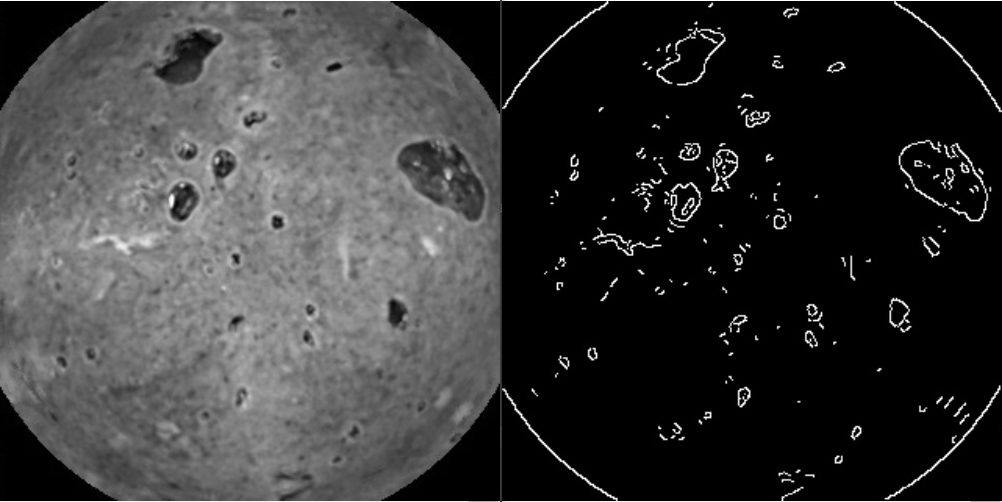
\includegraphics[scale=0.5]{cannyedge}
	\centering
	\caption{Ukázka Cannyho detektoru z průběhu práce}\label{fig:cannyedge}
\end{figure}


\section{Aktuální stav trhu}
\subsection{Rapid Software v8}
Rapid Software v8 je vyvinut společností Given Imaging, která mimo jíné vyrábí i kamery PillCam SB3. Jejich software je proto dodáván s těmito kamerami. Software umí spoustu užitečných věcí, ale pro charakter této práce je pouze podstatné, že nabízí detekci krve ve střevech. Škoda, že výrobce již neudává s jakou přesností. Na obrázku \ref{fig:rapid} je vidět ukázka rozhraní.\cite{pillcam}

\begin{figure}[h]
	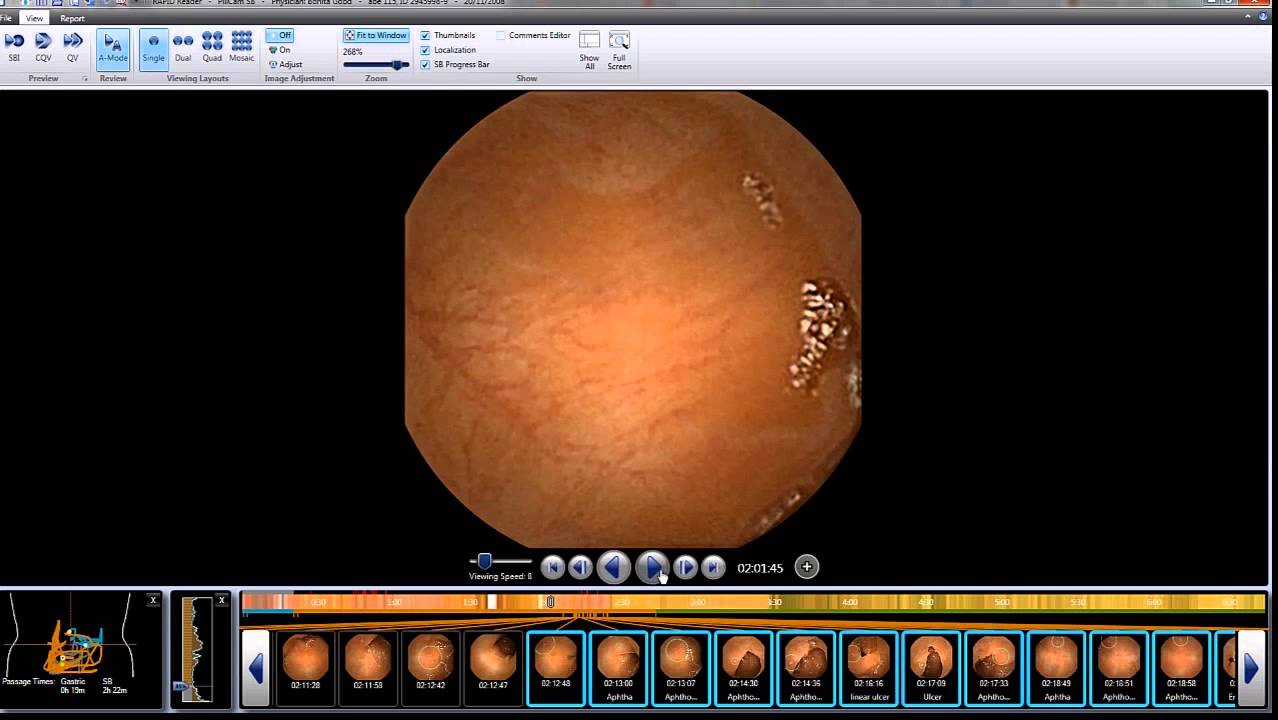
\includegraphics[scale=0.25]{rapid}
	\centering
	\caption{Ukázka Rapid v8\cite{rapidsoftware}\label{fig:rapid}}
\end{figure} 
\FloatBarrier

\subsection{Endocapsule 10 System}
Endocapsule 10 System je software vyvinutý společností Olympus, který ho také dodává ke svým kamerám. Software mimo základních věcí má algoritmy pro detekci červené barvy, bublin, nečistot a stejných obrázků. Díky těmto algoritmům je možné odfiltrovat nezajímavé či nehodnotné obrázky a nemusí se tak procházet celý vzorek. Ukázka rozhraní je vidět na obrázku \ref{fig:olympus}.\cite{endocapsule}

\begin{figure}[h]
	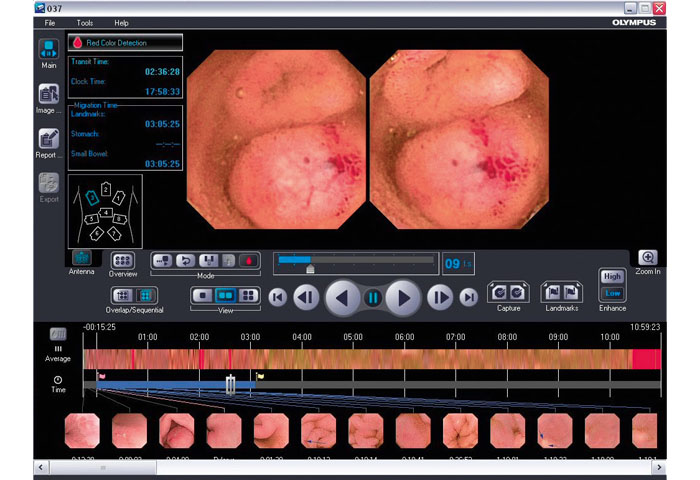
\includegraphics[scale=0.5]{olympus}
	\centering
	\caption{Ukázka Endocapsule 10 System \cite{olympuseuropa}\label{fig:olympus}}
\end{figure}
\FloatBarrier

\subsection{MiroView 2.5}
MiroView 2.5 je software vyvinutý společností IntroMedic, která taktéž dodává řešení se svými kamerami. Poskytuje základní funkcionalitu práce s videem a nabízí také automatickou detekci krve. Na obrázku \ref{fig:miroview} je vidět ukázka rozhraní.\cite{intromedic}

\begin{figure}[!h]
	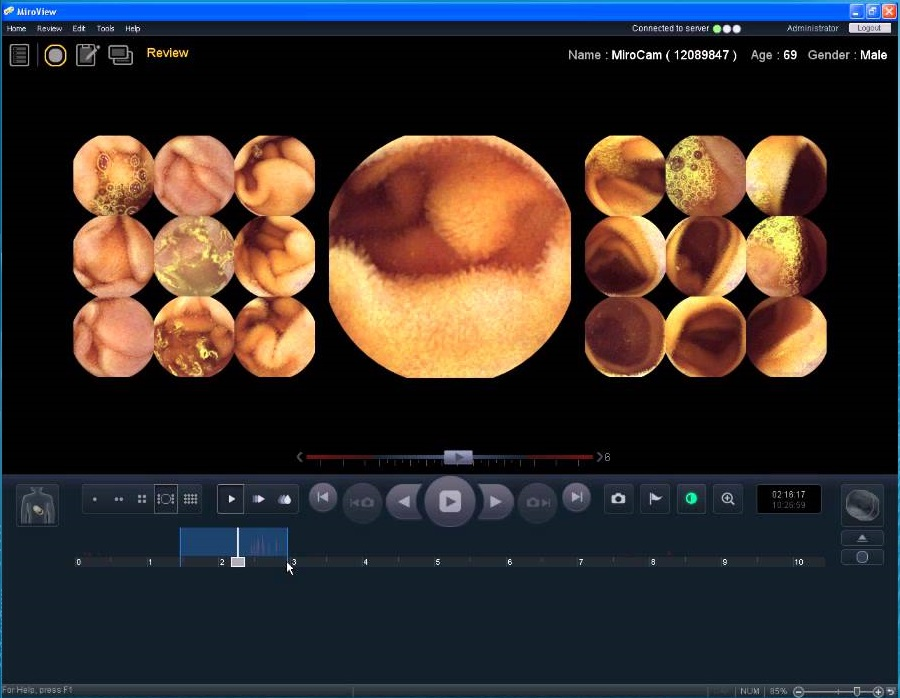
\includegraphics[scale=0.7]{miroview}
	\centering
	\caption{Ukázka MiroView 2.5\cite{miroview}\label{fig:miroview}}
\end{figure} 
\FloatBarrier
\clearpage
\subsection{GISentinel}
GISentinel je software vyvinutý společností Xyken ve spolupráci s Mayo Klinikou\footnote{Jedna z nejlepších klinik v USA, mimo jiné se také soustředí na výzkum. Spolupracuje i s ČR.\cite{about}}. Jejich software umí detekovat krev, polypy a vředy. Je k dispozici také na platformu Android, což umožňuje značnou mobilitu. Ukázka rozhraní je vidět na obrázku\ref{fig:gisentinel}.\cite{gisentinel}

\begin{figure}[h]
	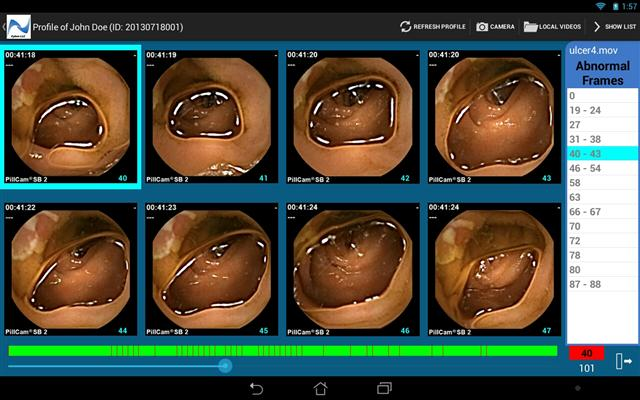
\includegraphics[scale=0.9]{gisentinel}
	\centering
	\caption{Ukázka GISentinel\cite{gisentinel}\label{fig:gisentinel}}
\end{figure}
\FloatBarrier
\begin{comment}
\section{Specifikace biomedicínských dat}
Data z kamer jsou získána, jako sled obrázků. Každý výrobce má svůj specifický vetšinou uzavřený formát. Ve všech případech se ale jedná o RGB data, která zaznamenává přímo kamera.
\end{comment}
	\chapter{Definice problému}
Hlavním problémem při zpracování dat z kapslové endoskopie je jejich nepřeberné množství. Lékaři musí projít obrázek po obrázku, což pro ně znamená velkou časovou náročnost. Ta by šla využít při řešení konkrétního problému jinak než jeho hledáním. Je proto potřeba nalézt takové řešení, které by tuto práci maximálně zjednodušilo a usnadnilo.

Vyvinutá aplikace by měla být schopná vyhodnotit záznam a detekovat možné krvácení ve střevech. Data z kamery jsou extrahována do proprietárního formátu každého výrobce, ze kterého pak lze extrahovat sekvenci nafocených obrázku buď do formátu \gls{glos:AVI}, ale s velkou kompresí, a tudíž ztrátou informací, anebo do sekvence po sobě jdoucích \gls{glos:JPG} obrázku beze ztráty kvality. Aplikace přijme tato data jako vstup. A na výstupu pak bude informace, zda se v daných datech nachází krvácení. 

\begin{figure}[h]
	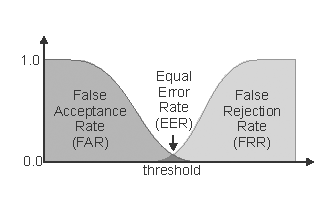
\includegraphics[scale=0.8]{eergraf}
	\centering
	\caption{EER graf \cite{gumption:}\label{fig:eergraf}}
\end{figure}

Je nutné popsat nebo definovat hledaný objekt tak, aby se za pomocí zpracování obrazu dal objekt nalézt s co největší přesností a nejmenším počtem chyb. Bylo by tedy potřeba nalézt \gls{glos:EER} mezi \gls{glos:FAR} a \gls{glos:FRR} viz obrázek, \ref{fig:eergraf}. Jelikož je v biomedicíně nutné nalézt všechny pozitivní objekty a ideální stav je 0\% \gls{glos:FRR}, tak se dá akceptovat větší míra \gls{glos:FAR}. Jinými slovy - je lépe označit více objektů, i když některý z nich může být chybou, než-li minout snímek, v němž se vyskytuje problém.

\begin{figure}[h]
	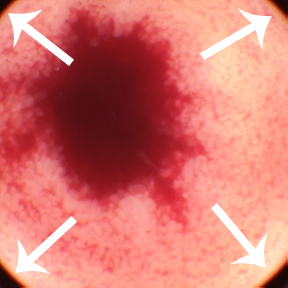
\includegraphics[scale=0.6]{anomalie}
	\centering
	\caption{Anomálie při sběru dat \label{fig:anomalie}}
\end{figure} 

Největším problémem je definování hledaného objektu, neboť kvalita dat není kvůli nízkému rozlišení kamer příliš velká. A navíc, každý výrobce má specifické barevné schéma, rozlišení a artefakty, které vznikají při sběru dat. Ukázkou může být obrázek \ref{fig:anomalie}, jenž znázorňuje, že tato kamera má u okrajů viditelný pruh barev, který pak může způsobovat problémy. V datech se také vyskytuje spousta anomálií, jež komplikují rozpoznávání objektu (různé odlesky, zbytky potravy, podobné barevné rozpoložení, …). Bude tedy potřeba zkombinovat více metod pro dosažení co nejlepšího výsledku.


V následujících kapitolách jsou uvedeny související vědecké práce, které se zabývají definováním stejného problému.

\section{Detection of bleeding in wireless capsule endoscopy using range ratio color \cite{detection}}
V článku „Detection of bleeding in wireless capsule endoscopy images using range ratio color“ výsledky byly klasifikovány na možnosti krvácení či neoznačení výskytu krve. Byla zde použita platforma C\#.

Analýza obrazu probíhala vždy ve dvou krocích. První krok efektivně rozdělí vstupní videa na ty, které obsahují výskyt krvácení a naopak. V druhém kroku následuje samotná detekce krvavých míst a klasifikace aktivních vzorků krvácení. První testovanou funkcí byla barva, která přinesla pouze selhání. Použitý algoritmus nepřinesl výsledky, které se očekávaly. Druhou testovací funkcí bylo použití parametrů poměr – barva. Tato funkce přinesla lepší výsledky než první. Oba dva algoritmy probíhaly téměř stejně - testovaly se všechny pixely na obrázku o proti podmínce, která se lišila v závislosti na použitém algoritmu. Podmínky je možné vidět na obrázku \ref{fig:clanekalg}.
\begin{figure}[h]
	
\includegraphics[scale=0.7]{clanekalg}
	\centering
	\caption{Použité algoritmy.\cite{detection} \label{fig:clanekalg}}
\end{figure} 

Bylo testováno 100 \gls{glos:WCE} snímků pořízených na různých částech trávícího traktu. Při použití stanovených podmínek byl výsledek první funkce s přesností stanoven na pouhých 48\%. Avšak druhá funkce umožnila povýšit přesnost až na 98\%. Přehled dosažených výsledků u obou metod můžeme shledat v tabulce \ref{tab:detection}.

\begin{table}[h]
	\centering
	\begin{tabular}{|l|c|c|c|c|}
		\hline
		\bf Klasifikace & \multicolumn{1}{l|}{\begin{tabular}[c]{@{}l@{}}\bf Detekovaných \\ \bf snímků s krví\end{tabular}} & \multicolumn{1}{l|}{\begin{tabular}[c]{@{}l@{}}\bf Detekovaných\\ \bf snímku bez krve\end{tabular}} & \multicolumn{1}{l|}{\begin{tabular}[c]{@{}l@{}}\bf Celková\\ \bf správná hodnota\end{tabular}} & \multicolumn{1}{l|}{\bf Přesnost} \\ \hline
		Pouze červená barva & 2 & 98 & 48 & 45\% \\ \hline
		Rozsah barev & 52 & 48 & 98 & 98\% \\ \hline
	\end{tabular}
	\caption{Výsledku algoritmů. Přeloženo z \cite{detection}}
	\label{tab:detection}
\end{table}
\FloatBarrier

Závěrem můžeme konstatovat, že tato metoda je jednoduchá a přesná.

\section{„A technique for blood detection in wireless capsule endoscopy images \cite{technique}}
Článek „A technique for blood detection in wireless capsule endoscopy images“ se zabývá způsobem rozlišování mezi běžnou sliznicí a regionů krvácejících tkání. Opět pomocí WCE snímků. Tohoto způsobu bylo dosaženo identifikaci lišících se oblastí. Lišit se mohou prostorové nebo spektrální charakteristiky od svého okolí. Oblasti pokryté krví jsou považovány za izolované cíle na pozadí. Celý tento proces je označen za detekce anomálií. 

Detekce anomálií se provádí prostřednictvím testování hypotéz daného problému. V případě detekce krve se používá pixel (anomální pixely) při reprezentaci barvy a stanovené hodnoty kovarianční matice. Vše se provádí za předpokladu stacionárního procesu v pozadí. Tento předpoklad se potlačuje především při výskytu vzduchových bublin či organických zbytků. Z tohoto důvodu je aplikován předzpracující stupeň – tedy příprava dat pro detekci anomálií a následně po dokončení spuštění RX algoritmu. Postup vícestupňové detekce krve je následující:

\begin{enumerate}
	\item Odstranění tmavých míst a detekce červených pixelů -
	V první fázi se vyloučí regiony, které nejsou detekovány jako užitečné (střevní šťávy, tmavé oblasti) a vyberou se pouze regiony s výskytem krve. Druhá fáze je rozdělena na další pod části. Nejprve se odstraní pixely tmavé velmi barvy, poté jsou červené pixely detekovány jako potencionální krev. Střevní obrazy dokáží poukázat na vysoce červený odstín. Výjimkou jsou snímky pořízené z oblasti tlustého střeva, kde jsou dominantní barvy oranžové až žlutozelené vzhledem k výskytu fekálních ostatků. 
	\item Hrana maskování -
	 Abychom snížili výskyt anomálií, aplikujeme okrajové maskování. Hrany jsou získány za pomocí Mumford-Stashova algoritmu jako výsledky funkční minimalizace problému. Obraz je dále předán dalšímu zpracování.
	\item Detekce krve -
	V tomto okamžiku jsou shromážděny výsledky z již předchozích fází. Kombinací těchto dvou způsobů třídění dat dosáhneme lepší spolehlivosti konečného výsledku. Kombinací detekcí červených barev, detekcí anomálií a maskováním získáme nekrvácející oblasti. 
	\item Morfologické operace -
	Krvácející oblasti se nejeví jako malé a izolované oblasti. Na základě tohoto faktu je užitečné odebrat izolované anomálie pixelů. Na obrázku \ref{fig:clanepostup} můžeme shledat konečnou podobu detekce krve.
\end{enumerate}

\begin{figure}[h]
	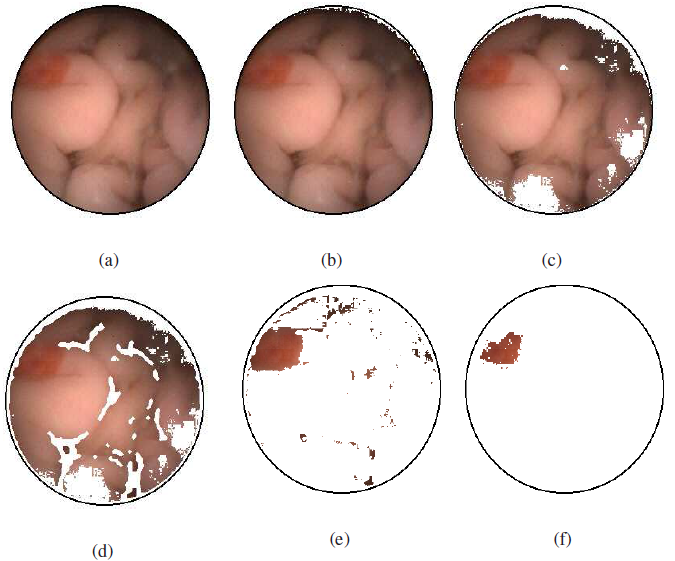
\includegraphics[scale=0.5]{clanekpostup}
	\centering
	\caption{Postup algoritmu a.originální obraz;b.odstranění černých pixelů;c.detekce červené barvy;d.maskování hran;e.detekce krve;f.výsledek RX algoritmu \cite{technique} \label{fig:clanepostup}}
\end{figure} 
\FloatBarrier
	
Simulace byly prováděny na 11 sekvencích (8 patologických případů, 3 zdraví jedinci). Každá sekvence se skládá ze 101 rámců o velikosti 256 x 256 pixelů. Přesnost výsledků byla hodnocena za pomocí standardních kriterií v biomedicíně (upřesněno v kapitole \ref{sec:metodologie}). Na obrázku \ref{fig:clanektabulka} můžeme shledat výkonnost navrhovaného algoritmu.

Výsledky ukázaly vyšší citlivost a specifičnost experimentálních navrhovaných způsobů. Tím pádem se dosahuje uspokojivých výsledků. Nesmí se však opomenout fakt, že použité sekvence jsou komprimovány. V důsledku komprimace dochází k negativnímu ovlivnění zaváděné komprese. Budoucí vývoj bude aplikovat konkrétní algoritmus na ověření nekomprimovaných dat a vykořisťování korelace mezi sousedními rámy a to vše za účelem zlepšení výkonu detekce.

\begin{figure}[h]
	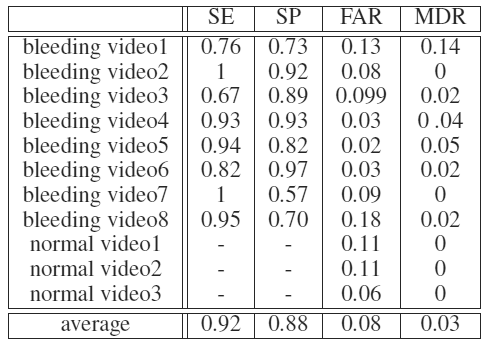
\includegraphics[scale=1]{clanektabulka}
	\centering
	\caption{Výsledky RX algoritmu \cite{technique} \label{fig:clanektabulka}}
\end{figure} 
\FloatBarrier

\section{Problémy detekce artefaktů v reálném prostředí}
Z vědeckých článků je zřejmé, že na vybrané databázi testovaných vzorků dosáhli celkem dobré úspěšnosti. Nicméně, nabízená řešení jsou příliš orientována na detekci dle barvy. V prvním případě se bude v reálných datech vyskytovat mnoho \gls{glos:FP}, protože na každém snímku se objeví alespoň jeden pixel, který bude zapadat do daného rozsahu.

V druhém článku je přidáno odstranění nechtěných anomálií po detekci barev. To může mít za následek zpřesnění výsledků, neexistuje zde však další mechanismus nezávisle na barvě, např. detekování samotného tvaru.

Z článku lze vycházet, jelikož přece jen detekce barvy je stěžejní pro určení krve. Pro přesnější výsledek je však nutné hledaný objekt definovat za pomocí detekce tvaru. Detekováním tvaru bude možné popsat rozdílnost od pozadí (lidský mozek zpracovává informace podobně, je schopný detekovat tvar objektu, aniž by záleželo na barvě).
	\chapter{Návrh softwarového řešení}
Pro softwarové řešení byla provedena základní analýza požadavků na systém, ze které se specifikovaly funkční a nefunkční požadavky. Na základě těchto požadavků bylo rozhodnuto o zvolených technologiích a architektuře softwaru.
\section{Analýza požadavků na systém}
Diagram užití, který je ztvárněn na obrázku, \ref{fig:usecase} je pro uživatele velice jednoduchý, protože aplikace má být intuitivní a slouží pouze k jednomu účelu a to zadání nové analýzy dat. Pro vývojáře bude nabízet možností více a to zejména ladění algoritmů.

\begin{figure}[h]
	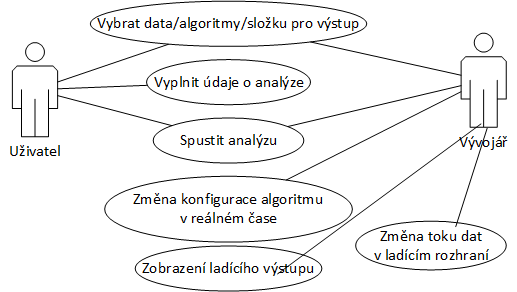
\includegraphics[scale=1]{usecase}
	\centering
	\caption{Diagram užití \label{fig:usecase}}
\end{figure} 

\subsection{Funkční požadavky}

\begin{table}[h]
	\centering
	\begin{tabular}{|
			>{}l |l|}
		\hline
		\multicolumn{1}{|c|}{\bf Funkční požadavek} & \multicolumn{1}{c|}{\bf Popis} \\ \hline
		\begin{tabular}[c]{@{}l@{}}Vybrání dat/algoritmů/\\ složky pro výstup\end{tabular} & \begin{tabular}[c]{@{}l@{}}Aplikace zobrazí dialog pro výběr dat, \\ algoritmů a složky pro výstup.\end{tabular} \\ \hline
		Vyplnění údajů o analýze & \begin{tabular}[c]{@{}l@{}}Aplikace nabídne formulář pro vyplnění\\ názvu a popisu analýzy.\end{tabular} \\ \hline
		Spuštění analýzy & Aplikace spustí analýzu dat. \\ \hline
		\begin{tabular}[c]{@{}l@{}}Změna konfigurace algoritmu\\ v reálném čase\end{tabular} & \begin{tabular}[c]{@{}l@{}}Aplikace umožní změnu konfigurace\\ algoritmů v reálném čase pro lepší\\ ladění algoritmů.\end{tabular} \\ \hline
		Zobrazení ladícího výstupu & \begin{tabular}[c]{@{}l@{}}Aplikace zobrazí ladící výstup aktuálně\\ zpracovávaného snímku, jako nové okno\\ s obrázkem snímku.\end{tabular} \\ \hline
		\begin{tabular}[c]{@{}l@{}}Změna toku dat v ladícím\\ rozhraní\end{tabular} & \begin{tabular}[c]{@{}l@{}}Aplikace umožní vývojářům přehrávat\\ již analyzované video, posouvat rychlost\\ přehrávání či vybrat konkrétní snímek.\end{tabular} \\ \hline
	\end{tabular}
	\caption{Funkční požadavky na aplikaci}
	\label{tab:funkcni}
\end{table}
\FloatBarrier
\subsection{Nefunkční požadavky}

\begin{table}[h]
	\centering
\begin{tabular}{|
		>{}l |l|}
	\hline
	\multicolumn{1}{|c|}{\bf Nefunkční požadavek} & \multicolumn{1}{c|}{\bf Popis} \\ \hline
	Intuitivní ovládání & \begin{tabular}[c]{@{}l@{}}Aplikace bude jednoduchá k použití\\ i bez manuálu.\end{tabular} \\ \hline
	Optimalizace & \begin{tabular}[c]{@{}l@{}}Aplikace musí zvládat zpracovávat\\ velké množství dat a být co\\ nejefektivnější.\end{tabular} \\ \hline
	Generování výstupních souborů & \begin{tabular}[c]{@{}l@{}}Aplikace bude umět generovat výstup\\ do předem zvolených formátů.\end{tabular} \\ \hline
	Multiplatformní použití & \begin{tabular}[c]{@{}l@{}}Aplikace by měla být nezávislá na \\ konkrétní platformě.\end{tabular} \\ \hline
\end{tabular}
\end{table}
\FloatBarrier

\begin{table}[h]
	\centering
	\begin{tabular}{|
			>{}l |l|}
		\hline
	Možnost implementace více GUI & \begin{tabular}[c]{@{}l@{}}Aplikace by měla být navržena tak, aby\\ bylo možné vystavět na ní různá rozhraní\\ např. desktop nebo web.\end{tabular} \\ \hline
	Oddělené prostředí & \begin{tabular}[c]{@{}l@{}}Vývojové prostředí bude oddělené od\\ produkčního, aby zbytečně nedocházelo k\\ nepředvídatelným chybám. Bude pouze\\ využívat část společné funkcionality.\end{tabular} \\ \hline
\end{tabular}
	\caption{Nefunkční požadavky na aplikaci}
	\label{tab:nefunkcni}
\end{table}


\section{Použité technologie a knihovny}
Tato kapitola se zabývá použitými technologiemi a knihovnami. Technologie byly zvoleny na základě autorových zkušeností s nimi a také vhodností pro charakter práce. Následující výčet ukazuje hlavní technologie použité v práci, mimo ně jsou ještě použity různé podpůrné knihovny od Apache, které již však nejsou klíčové pro funkčnost a spíše usnadňují práci.
\begin{itemize}
	\item Java - objektově orientovaný programovací jazyk vyvinutý společností Sun Microsystems a později odkoupen společností Oracle. Java je multiplatformní jazyk, tudíž není problém spustit jeden kód na více operačních systémech či zařízení. V práci je použita Java 1.8\_0.45 a je tak minimální podporovanou verzí pro spuštění software. V práci jsou využity nejmodernější přístupy, které Java 1.8 přináší.
	\item JavaFX8 - technologie pro tvorbu bohatých klientských aplikací. Je jednou z možných implementací \gls{glos:GUI} aplikace (více o \gls{glos:GUI} v kapitole \ref{sec:arch}). Od verze Javy 1.8 je již standardem pro tvorbu \gls{glos:GUI} a nahrazuje starý swing.
	\item OpenCv - knihovna pro počítačové vidění pod licencí BSD. Knihovna nabízí mnoho nástrojů pro práci s obrazovými daty a je vysoce optimalizovaná pro produkční aplikace. Využívá nativní kód přímo pro určité platformy a hardwarovou akceleraci pomocí OpenCL, pokud je možná. Je hlavním nástrojem pro výpočty a manipulaci s obrazem, v Jave jsou napsány pouze minoritní výpočetní operace\cite{learning}
	\item Apache Maven - nástroj pro sestavování programu, řešení automatických závislostí na knihovny a správy modulů projektu.\cite{maven}
	\item Apachae POI - knihovna pro manipulaci různých formátů založených na Office Open XML standars a Microsoft OLE 2 Compound Document format. Lze tak vytvářet a pracovat se soubory XLS a XLSX, případně číst další soubory vytvořené z Microsoft Office.\cite{apache-1}
	\item Apache PDFBox - knihovna, která umožňuje vytvářet PDF dokumenty, manipulovat s existujícími a získávat obsah dokumentů.\cite{apache-2}
	\item ProGuard - nástroj, který minimalizuje, optimalizuje, obfuskuje a před ověřuje Java třídy. Umí detekovat a odstranit nepoužívané třídy, pole, metody a atributy pro zmenšení výsledného kódu. Optimalizuje bytecode a odstraňuje nepoužívané instrukce. Přejmenovává zbývající třídy, pole a metody použitím krátkých nevýznamných jmen, aby nebylo jednoduché program dekompilovat. Přeznačuje a před ověřuje existující třídy pro Java 6 a vyšší, aby tak zrychlil jejich načítání.\cite{proguard} V práci je použit jako plugin do Mavenu při sestavování programu.
	\item Launch4J - nástroj pro obalování spustitelného Java programu nativním kódem pro Windows a vytváření tak .exe souborů. Nástroj také umožňuje definování minimálního JRE a případě přesměrování na stránky pro stažení případně je možné vložit celé JRE, jako knihovnu, kterou nástroj bude načítat pří spuštění programu.\cite{launch4j} V práci je použit jako plugin do Mavenu při sestavování programu.
\end{itemize}

\section{Vývoj algoritmů}
K zjištění přítomnosti krve v trávícím traktu nebylo možné použít stejné principy pro všechny možné případy výskytů krvavých oblastí. Proto byly vyvinuty dva algoritmy pro detekci velkých a malých skvrn, které používají víceméně stejné metody, ale odlišné postupy. Jediná stejná část pro oba dva algoritmy je, že se na začátku zpracování ořízne obraz kvůli vznikajícím barevným anomáliím na okrajích snímací části kamery.
Popis algoritmů je zde obecný bez použití konkrétních nakonfigurovaných hodnot, v příloze \ref{sec:prilohaKonfig} a \ref{sec:prilohaHodnoty} jsou vidět konkrétní hodnoty a jejich vysvětlení.
\subsection{Detekce malých skvrn}
Algoritmus je rozdělen na dvě nezávislé částí, které se pak na konci porovnají, a v případě schody se snímek vyhodnotí pozitivně.

První část je zaměřena na filtrování obrazu dle určitého barevného rozmezí, která je zpřesněna dalšími technikami.
\begin{enumerate}
	\item Převod barevného formátu z BGR do HSV. S HSV formátem je možné přesněji vyjádřit barevné rozmezí, které je potřeba zachovat, viz obr. \ref{fig:alg_1}.E.
	\item Filtrace matice dle definovaného barevného rozmezí. Výsledkem operace je nová matice, která obsahuje pouze vybrané barvy a jejich hodnoty jsou reprezentovány jako binární data, dochází tedy ke ztrátě barevné informace, viz obr. \ref{fig:alg_1}.F.
	\item Pro všechny spojité oblasti, které vznikly z předchozího kroku, se vypočte jejich oblast a ponechají se pouze ty, které jsou větší než definovaná hodnota. Tím dojde k odstranění nevýznamných miniaturních oblastí, které jsou pravděpodobně vzniklé šumem, případě jinými anomáliemi. A také se vyplní nevybarvené oblasti uvnitř spojitých oblastí, viz obr. \ref{fig:alg_1}.G.
	\item Na všechny body s hodnotou 1 ve vyfiltrované matici se zkopíruje barevná informace z původní HSV matice, tím se vrátí barevná informace k dalšímu zpracování, viz obr. \ref{fig:alg_1}.H.
	\item Provede se morfologická operace dilatace dle zadané konfigurace. Tím dojde ke spojení všech blízkých bodů v matici a vzniknou tak větší spojité oblasti, kde by potencionálně mohla být krev, viz obr. \ref{fig:alg_1}.I.
	\item Pro všechny spojité oblasti, které vzniknou po dilataci, se vypočte jejich ohraničující čtverec, který se vyřízne z matice.
	\item V každém takto vzniklém čtverci se provede znovu filtrování dle barvy, ale s jinou "přisnější" konfigurací. V nově vzniklé matici už se nefiltrují malé artefakty a provede se rovnou dilatace. To má za následek, že se v podstatě nic nezmění, nebo se čtverec rozpadne na více oblastí, anebo dojde k vyřazení čtverce z potencionálních detekovaných oblastí.
	\item V každém takto upraveném čtverci se najdou všechny spojité oblasti, ohraničí se čtvercem a uloží se do pole, které v sobě drží ostatní \gls{glos:ROI}, viz obr. \ref{fig:alg_1}.J.
\end{enumerate}

\begin{figure}[h]
	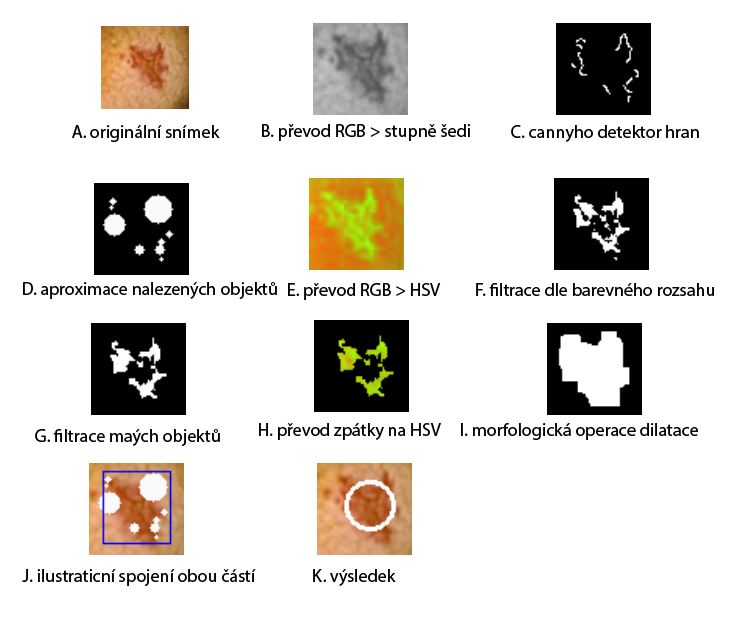
\includegraphics[scale=0.5]{alg1}
	\centering
	\caption{Ukázka průchodu algoritmu detekce malých skvrn. \label{fig:alg_1}}
\end{figure} 
\FloatBarrier

V druhé části algoritmu se detekují hrany a určí se tak potencionální objekty, které jsou odlišné od pozadí. Postup je následující:
\begin{enumerate}
	\item Převod barevného formátu z GRB na odstíny šedi, jelikož je k detekci hran vhodnější, viz. obr. \ref{fig:alg_1}.B.
	\item Gaussovo rozmazání dle definované konfigurace.
	\item Cannyho detektor hran dle definované konfigurace, viz. obr. \ref{fig:alg_1}.C.
	\item Pro všechny spojité nalezené hrany se vypočte minimální obklopující kružnice. Ta slouží, jako jednoduchá aproximace hledaného objektu.
	\item Jelikož vznikají anomálie při detekci hran a zejména okrajové části kamery jsou často zahrnuty ve výsledku, tak je nutné vybrat pouze ty kružnice, které nepřesahují maximálně definovaný průměr. Je v podstatě nemožné, aby se tímto odstranila hrana, která se nemá odstranit, protože tento algoritmus detekuje pouze menší skvrny a anomálie, které vznikají jsou velmi velké.
	\item Zanesení zbylých kružnic do pomocné matice, viz. obr. \ref{fig:alg_1}.D.
\end{enumerate}

Jakmile jsou k dispozici obě části algoritmu, tedy matice, která obsahuje pomocné kružnice, a list všech \gls{glos:ROI}. Tak dojde k vyhodnocení, zda-li je matice pozitivní. To je provedeno iterací přes všechny čtverce v listu a pokud se v oblasti konkrétního čtverce nachází alespoň jeden bod z kružnice, tak je místo pozitivní, viz obr. \ref{fig:alg_1}.K.


\begin{figure}[h]
	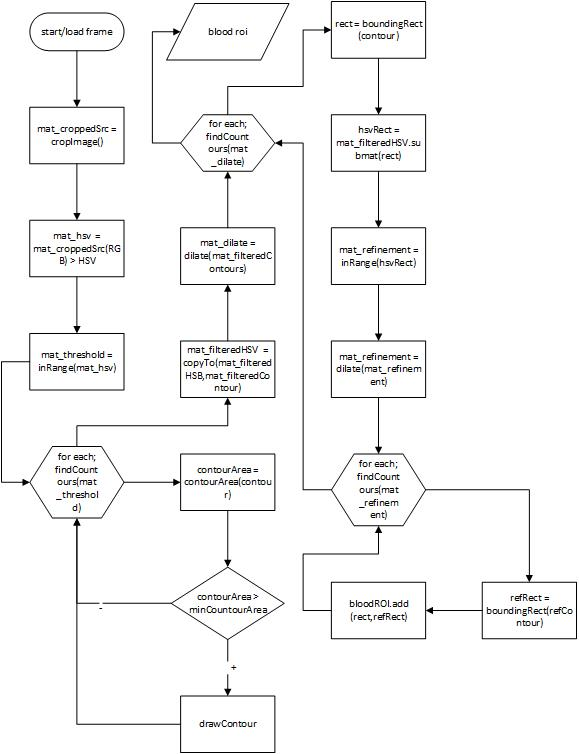
\includegraphics[scale=1]{sb_diagram_1}
	\centering
	\caption{Vývojový diagram první části algoritmu detekce malých skvrn. \label{fig:sb_diagram_1}}
\end{figure} 
\FloatBarrier

\begin{figure}[h]
	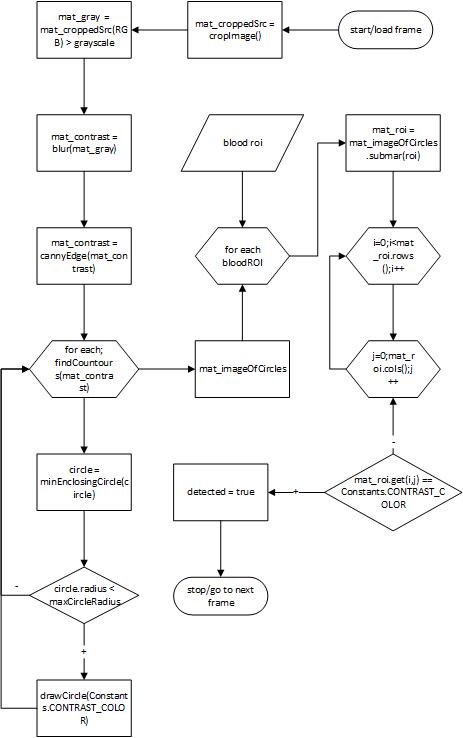
\includegraphics[scale=1]{sb_diagram_2}
	\centering
	\caption{Vývojový diagram druhé části algoritmu detekce malých skvrn a spojení obou částí. \label{fig:sb_diagram_2}}
\end{figure} 
\FloatBarrier


\subsection{Detekce velkých skvrn}
Konstrukce druhého algoritmu je značně jednodušší a přímočařejší než-li detekce menších skvrn. Jedná se o nalezení velké oblasti se stejným barevným spektrem. Postup je následující:

\begin{enumerate}
	\item Převod barevného formátu z BGR do HSV, viz obr. \ref{fig:alg_2}.B.
	\item Filtrace matice dle definovaného barevného rozmezí, viz obr. \ref{fig:alg_2}.C.
	\item Filtrování miniaturních částí, viz obr. \ref{fig:alg_2}.D.
	\item Morfologická operace dilatace, viz obr. \ref{fig:alg_2}.E.
	\item Pro všechny spojité oblasti v matici se zjistí jejich plocha. Ta se porovná proti definované procentuální velikosti celkové oblasti a pokud je větší, tak se rámec vyhodnotí pozitivně. Např. pokud je spojitá oblast větší než-li 15\% celkové oblasti, viz obr. \ref{fig:alg_2}.F.
\end{enumerate} 

\begin{figure}[h]
	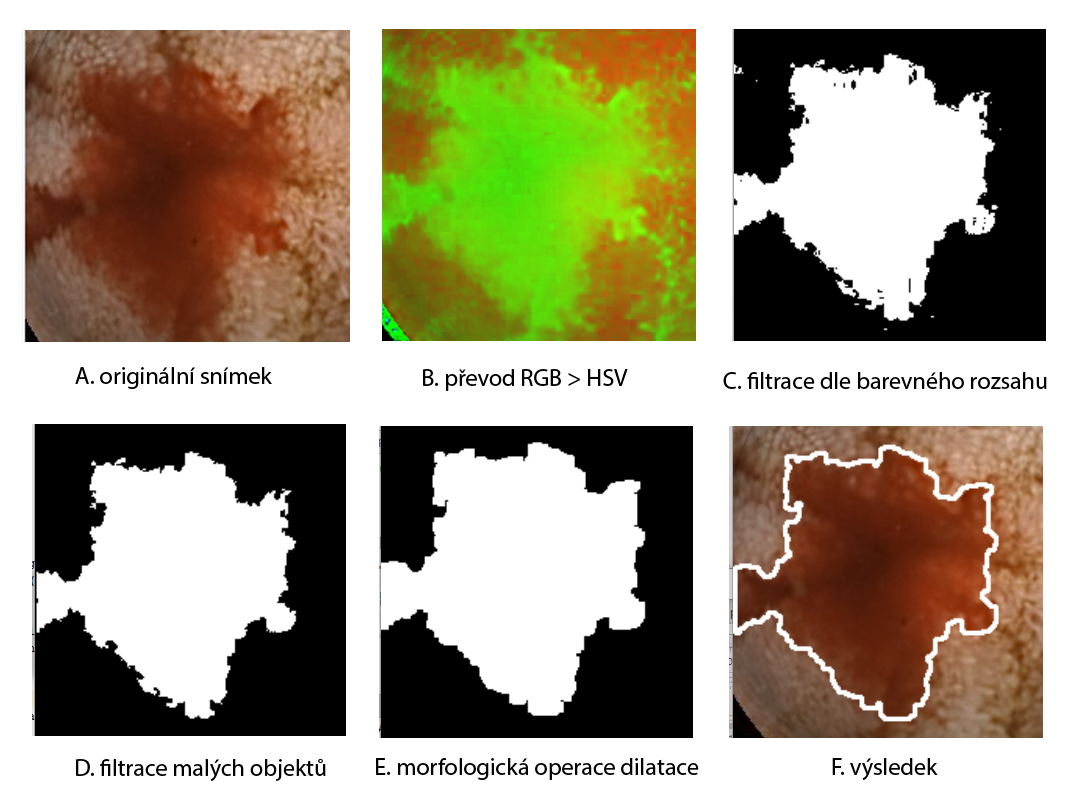
\includegraphics[scale=0.3]{alg2}
	\centering
	\caption{Ukázka průchodu algoritmu detekce velkých skvrn. \label{fig:alg_2}}
\end{figure} 


\begin{figure}[h]
	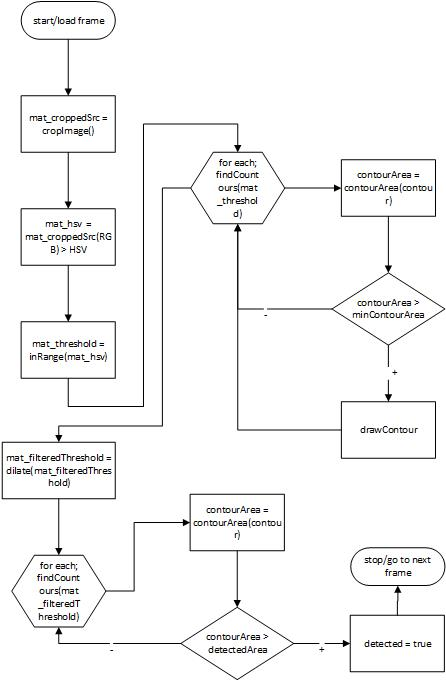
\includegraphics[scale=1]{bb_diagram}
	\centering
	\caption{Vývojový diagram algoritmu velkých skvrn. \label{fig:bb_diagram}}
\end{figure} 
	\chapter{Implementace software}
Software je rozdělen na čtyři moduly. Každý modul v sobě uzavírá specifickou funkcionalitu. Hlavním modulem je modul core, kde je veškerá logika programu. Ostatní moduly už jsou jen pro uživatelské rozhraní, které je případně možné implementovat i jinak např. je možné udělat webové rozhraní.
\section{Modul Core}
Modul core je jádro celého programu, uzavírá v sobě funkcionalitu pro načítání algoritmů, práci s obrazem, generování výstupních souboru a práci s více vlákny. Na obrázku \ref{fig:core_whole} je vidět základní schéma modulu. Modul je rozdělen do několika balíčku, z nichž stěžejní jsou algorithm, video, task a output. Ostatní balíčky obsahuje pomocné třídy, jako jsou různé utility třídy, DTO, vyjímky, ...

V modulu core je ještě několik tříd, které nejsou zařazené do žádného balíčku. Třída EnvLoader má na starost správné načtení konkrétních knihoven pro danou platformu, jelikož knihovna OpenCV využívá nativní knihovny zkompilované pro každou platformu zvlášť a v Jave jsou tyto knihovny volány přes \gls{glos:JNA}, tak je nutné načíst nativní knihovny do systému. Momentálně je v programu podporována platforma Windows x86 a x64.

Další třídou je BMAThreadFactory, která implementuje rozhraní ThreadFactory. Třída slouží, jako factory pro executor servise. Vlákna, která se zde vytvoří, jsou řazena pod jednu skupinu a ta může mít svůj volitelný název. Všechna vlákna jsou pak vytvořena s prioritou normal a neběží v režimu "démon". Veškerá práce s vlákny v programu pak probíhá pomocí ExecutorService, kde je využito BMAThreadFactory pro tvorbu nových vláken.

\begin{figure}[h]
	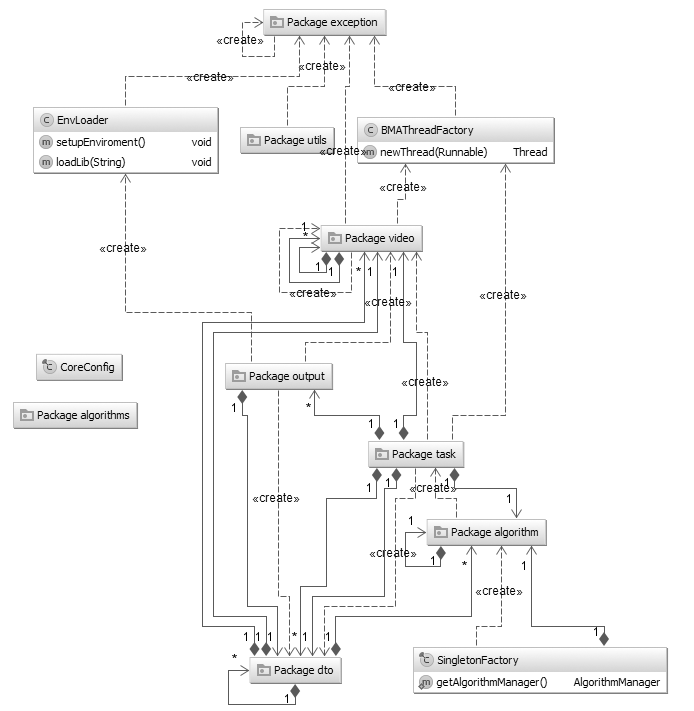
\includegraphics[scale=1]{core_whole}
	\centering
	\caption{Modul core \label{fig:core_whole}}
\end{figure} 
\FloatBarrier
\subsection{Balíček Algorithm}
V balíčku algorithm, jehož schéma je vidět na obrázku \ref{fig:core_algorithm}, je funkcionalita pro načítání počáteční konfigurace algoritmu a práci s načteními algoritmy. Veškerou funkcionalitu balíčku v sobě uzavírá třída AlgorithmManager, přes kterou se volá AlgorithmService a také v sobě drží aktuálně načtené algoritmy. V programu se vytváří pouze jedna singleton instance manageru a ta se pak získává přes SingletonFactory.

\begin{figure}[h]
	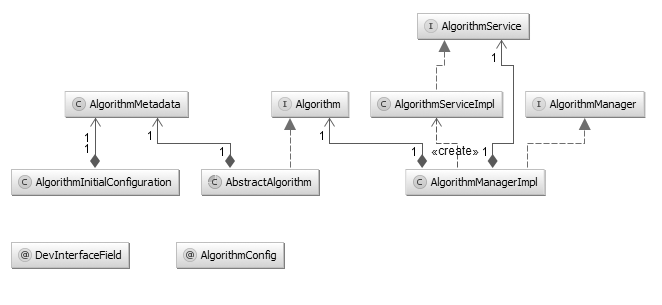
\includegraphics[scale=0.8]{core_algorithm}
	\centering
	\caption{Balíček algorithm \label{fig:core_algorithm}}
\end{figure} 
\FloatBarrier
Pro vytvoření nového algoritmu je nutné, aby nová třída implementovala rozhraní Algorithm nebo dědila již od základní implementace AbstractAlgorithm. Dále může volitelně obsahovat třídu, která slouží jako konfigurace algoritmu. Tato třída musí mít anotaci AlgorithmConfig. V konfiguraci je pak možné anotovat jednotlivé atributy anotací DevInterfaceField, ty pak budou na základě konfigurace v anotaci vidět ve vývojovém rozhraní. Konkrétní nastavení algoritmu je uloženo v externím XML souboru, který je mapován na třídu AlgorithmInitialConfiguration. Díky tomu je možné mít více algoritmů s různou konfigurací. Ukázka nového algoritmu je zobrazena na obrázku \ref{fig:core_new}. Načtení algoritmu pak probíhá následovně:
\begin{enumerate}
	\item Procházení všech XML souborů.
	\item Soubor je rozmaršálován na třídu AlgorithmInitialConfiguration pomocí JAXB.
	\item Pomocí reflexe je nalezena a vytvořena nová instance třídy, která je uvedena v className, viz. obrázek \ref{fig:core_new}.
	\item Nastavení metadat algoritmu.
	\item Vytvoření nové konfigurace algoritmu a nastavení atributů na základě hodnot v XML. Vše je pak dosazeno do instance třídy pomocí reflexe.
	\item Vložení inicializovaného algoritmu do mapy k ostatním algoritmům.
\end{enumerate}

\begin{figure}[h]
	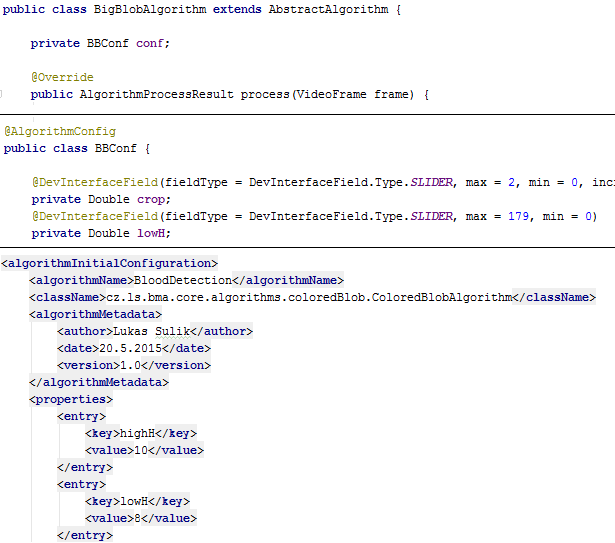
\includegraphics[scale=0.9]{core_new}
	\centering
	\caption{Ukázka nového algoritmu \label{fig:core_new}}
\end{figure} 
\FloatBarrier

\subsection{Balíček Video}
V balíčku video jsou pouze dvě třídy: Buffer a VideoFrame. VideoFrame je třída, která slouží k uchovávání informace o jednom obrazovém rámci. Má v sobě matici, která reprezentuje obrázek, číslo rámce a zámek. Zámek je zde proto, že se s rámcem pracuje ve více vláknech a je nutné poznat, zdali už byl rámec zpracován všemi algoritmy. Zámek je vyjádřen třídou AtomicInteger a je to číselná hodnota, která se nastavuje vždy při vytváření rámce (popsáno níže), a jedná se o vyjádření počtu algoritmů, které s ním budou pracovat. Po zpracování algoritmem se hodnota zámku sníží o jedna. VideoFrame také obsahuje pomocnou funkcionalitu pro vývojové rozhraní, tato funkcionalita je aktivní pouze pokud je vývojové rozhraní aktivní. Vývojová funkcionalita umožňuje dočasně ukládat matice z průběhu zpracování algoritmu do mapy, ale tato možnost funguje pouze pro jedno vlákno.

Třída Buffer slouží, jak již název napovídá, jako zásobník pro VideoFrame. Samotný zásobník je řešen pomocí rozhraní ConcurrentNavigableMap a konkrétní implementace ConcurrentSkipListMap. S touto třídou je možno pracovat na více vláknech bez rizika deadlocku. Pořadí hodnot v mapě je tříděno přirozeně pomocí klíče a datová struktura skip list umožňuje rychlé vyhledávání v mapě dle klíče. Velikost bufferu se dá řídit definovanou konstantou, po naplnění bufferu nelze přidávat další elementy. To zajišťuje metoda addFrame, která slouží pro vytvoření a vložení nového framu, pokud je již buffer naplněn tak nelze nový frame přidat. Čištění bufferu probíhá automaticky. Při vytvoření objektu je spuštěna čistící sekvence, která odmazává všechny framy s nulovou hodnotou zámku. Sekvence běží do té doby, než je buffer uzavřen a je prázdný. Uzavření bufferu je stav, kdy už do něj nelze přidat další hodnoty, stav je reprezentován atributem typu boolean.

\subsection{Balíček Task}
Další částí programu je balíček Task, jehož schéma je vidět na obrázku \ref{fig:core_task}. Třídy v něm obsažené slouží k vykonávání asynchronních úkolů a implementují buď Runnable nebo Callable, v případě, že je potřeba čekat na výsledek. V třídách grabber je načítání souborů z disku. Jak název napovídá tak buď videa, anebo celé složky (kde se načítají obrázky). K načtení je v obou případech použita knihovna OpenCV, která načte jednotlivé soubory a udělá z nich matice ve formátu BGR (pouze přeházené kanály o proti RGB, jinak je formát stejný). Načtená matice je pak vložena do třídy buffer, kde bude čekat na další zpracování.

Pro zpracování videa se využívá třída AlgorithmTask, která je potomkem AbstractBufferTask. V této třídě dochází ke zpracování dat algoritmem, metody pro sběr dat jsou definovány v abstraktním předkovi. Po vytažení dat se spustí metoda algoritmu, která zjistí, jestli se v konkrétním snímku nachází nějaká anomálie. V případě pozitivního výsledku se snímek uloží do přepravky, která se pak použije při generování výstupu. Jakmile je operace dokončena, z video snímku se odstraní zámek pro konkrétní algoritmus a pošle se signál pro aktualizaci průběhu.

\begin{figure}[h]
	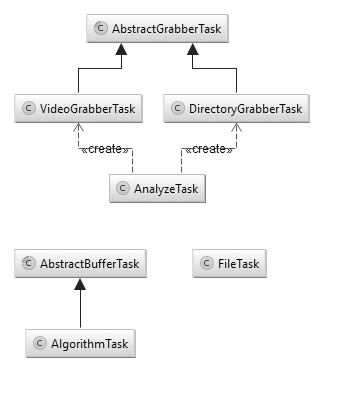
\includegraphics[scale=0.9]{core_task}
	\centering
	\caption{Balíček Task \label{fig:core_task}}
\end{figure} 
\FloatBarrier

Třída AnalyzeTask spojuje funkcionalitu všech předchozích tasku. Pro každý soubor se vytvoří buffer a spustí se GrabberTask na novém vlákně. Jakmile je GrabberTask zapnut, tak se vyžádají od AlgorithmManagera všechny aktivní algoritmy a jejich tasky, kde se použije tentýž buffer. Ty se poté také spustí asynchronně. Z důvodu optimalizace bylo přidáno omezení na zpracování maximálně dvou souborů/složek zároveň. I to ale občas může způsobovat problémy, tak do budoucího rozvoje práce by bylo dobré zlepšit optimalizace, např. použít knihovnu MapDB. Po dokončení všech operací se pošle signál k aktualizaci průběhu a vygeneruje se přepravka s výsledky analýzy.

\subsection{Balíček Output}
Poslední hlavní částí modulu Core je balíček output. Ten má v sobě obsaženou logiku pro generování výstupních souborů. V současné době je podporován formát XLSX a PDF. Generováni obou formátů je řešené podobně, každý formát však obsahuje specifické nástroje pro tvorbu. Schéma pro tvorbu XLSX je vidět na obrázku \ref{fig:core_output}. Aplikace komunikuje s generátory pomocí rozhraní FileOutput. V rámci generování XLSX(i PDF) se vnitřní logika rozpadne na několik menších generátorů, které implementují rozhraní XLSXGenerator (případně PDFGenerator). Tyto generátory se pak spustí v hlavní třídě XLSXOutput v předem daném pořadí a vznikne tak výsledný soubor.

\begin{figure}[h]
	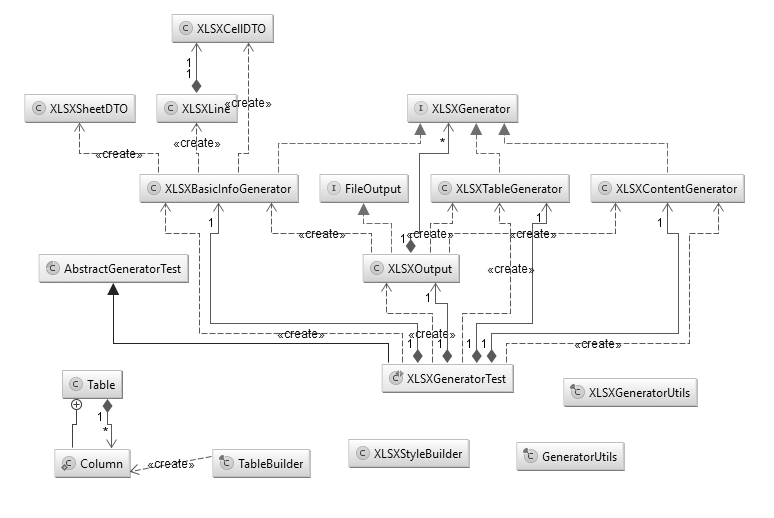
\includegraphics[scale=0.8]{core_output}
	\centering
	\caption{Schéma generátoru XLSX \label{fig:core_output}}
\end{figure} 
\FloatBarrier

Tento balíček obsahuje, jako jediný, jednotkové testy. Je zde vytvořen mock proběhnuté analýzy a podle něj jsou generovány soubory. Testy ale nejsou spouštěny při sestavování programu, spíše jsou zde pro ulehčení a zrychlení vývoje.


\section{Modul Fxml}
Modul FXML je pomocný modul pro práci s JavaFX, který pak dále využívá modul Application a Dev. Obsahuje pouze několik společných třídy pro tyto dva moduly, schéma je vidět na obrázku \ref{fig:fxml_whole}. JavaFX vytváří \gls{glos:GUI} pomocí speciálního XML formátu FXML nebo je možné využít i programátorský přístup a udělat vše manuálně. Pro vytvoření nového prvku je potřeba znát název FXML souboru a také jeho kontrolor, aby se nemuselo pokaždé tyto dvě věci definovat, tak třída FXApplication obsahuje metody pro tvorbu nových prvků a přepínání kontextu. Stáčí tedy definovat nový prvek v enumu FXMLElement a zavolat patřičnou metodu v FXApplication. Ta vezme prvek z enumu a pomocí FXMLCreator vytvoří nový prvek, k němuž je pak přiřazen abstraktní kontrolor. Jediná podmínka je pak ta, že každý kontrolor musí být potomkem abstraktního předka a v aplikaci pak proběhne přetypování na konkrétní kontrolor.

\begin{figure}[h]
	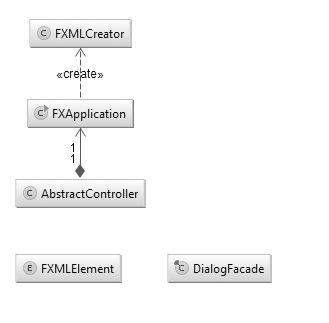
\includegraphics[scale=0.9]{fxml_whole}
	\centering
	\caption{Schéma modulu FXML \label{fig:fxml_whole}}
\end{figure} 
\FloatBarrier

Při vytváření elementu ve třídě FXMLCreator se také nastavuje cesta k lokalizačním souborům, ta se bere z MessageUtils, který je v modulu Core. Aplikace je tímto uzpůsobena na možnost více jazyků. V této třídě je možné vytvořit i element, který bude spolupracovat s \gls{glos:CDI}. Toho bylo využito téměř po celou dobu vývoje aplikace a byla zvolena implementace WeldSE. Ale po problémech s pomalejším načítáním programu a pro zvláštní chování s použitím ProGuard a Shade pluginu pro Maven bylo od této implementace opuštěno (funkce těchto pluginů je popsána v kapitole \ref{sec:app}). Tímto bohužel aplikace ztratila interceptory pro kontrolování výkonu jednotlivých metod, snazší logování programu pomocí log4j, řešení automatických závislostí a lepší práci se singletone objekty. Do dalšího možného vývoje práce je možné zkusit CDI implementovat pomocí Spring Boot, který by neměl dělat problémy, které vznikaly při použití WeldSE. A to zejména proto, že není definován pomocí XML, ale konfigurace se provádí přímo v Jave.

\section{Modul Application}\label{sec:app}
V modulu Application je definováno uživatelské rozhraní a komunikace s modulem Core. Aplikace je založena na návrhovém vzoru \gls{glos:MVC}. Jedná se pouze o několik kontrolorů a pomocných tříd, bez žádné složitější logiky, tu pak obstarává modul Core. Hlavním kontrolorem je třída MainController, jehož rozhraní je vidět na obrázku \ref{fig:app_main}. Práce s programem je zobrazena na obrázku \ref{fig:flow}.

\begin{figure}[h]
	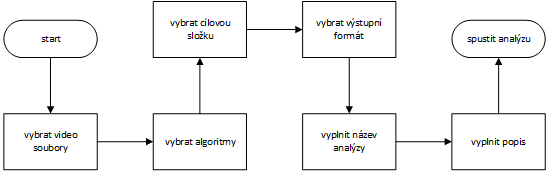
\includegraphics[scale=0.9]{flow}
	\centering
	\caption{Průběh práce s programem \label{fig:flow}}
\end{figure} 
\FloatBarrier

\begin{figure}[h]
	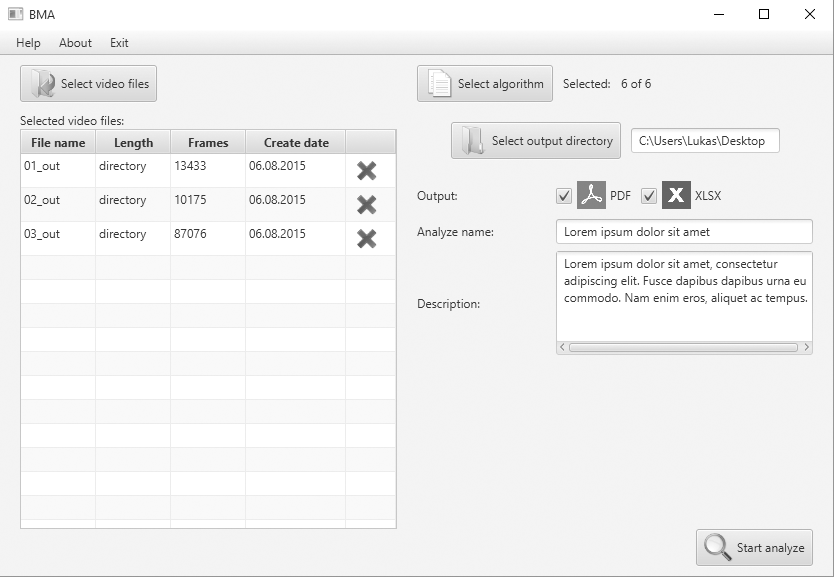
\includegraphics[scale=0.7]{app_main}
	\centering
	\caption{Hlavní obrazovka aplikace \label{fig:app_main}}
\end{figure} 
\FloatBarrier


Z hlavní obrazovky se dá spustit AlgorithmManagerController, viz. obrázek \ref{fig:app_manager}. Kde se vyberou konkrétní algoritmy, které se mají použít pro aktuální analýzu. Dále se na hlavní obrazovce dá zvolit, které soubory se budou zpracovávat a kam se pak vygenerují výstupní soubory. Lze k analýze připsat i volitelné doplňkové údaje, ty se pak také vygenerují k výstupním souborům. Po spuštění analýzy je zobrazen dialog průběhu, který je vidět na obrázku \ref{fig:app_progress}.

\begin{figure}[h]
	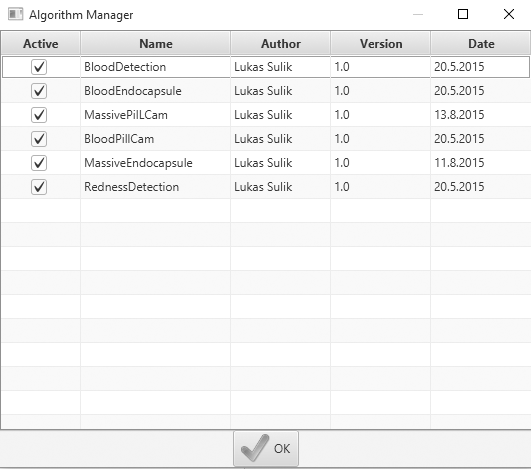
\includegraphics[scale=0.9]{app_manager}
	\centering
	\caption{Správa algoritmů \label{fig:app_manager}}
\end{figure} 
\FloatBarrier

ProgressDialogController implementuje rozhraní ProgressNotifier z modulu Core. Přes toto rozhraní jsou posílány signály z asynchronního zpracování souborů a na základě toho je v tomto případě aktualizováno uživatelské rozhraní. Při implementování jiného \gls{glos:GUI} je možné využít toto rozhraní jinak, např. pokud by se jednalo o webovou aplikaci, tak je možné ukládat záznam o průběhu do databáze a uživatel by se pak na něj mohl dotazovat pomocí ajaxových dotazů.

\begin{figure}[h]
	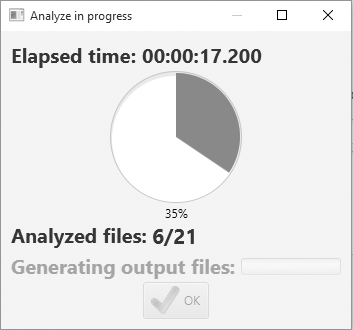
\includegraphics[scale=0.9]{app_progress}
	\centering
	\caption{Dialog průběhu \label{fig:app_progress}}
\end{figure} 
\FloatBarrier

V modulu application jsou umístěné Maven skripty pro sestavování programu. Nejprve je využit Maven Shade plugin, který dle definice autoru - "Tento plugin má schopnost zabalit program do uber-jar, včetně jeho závislostí a zastínit ho - tj. přejmenovat balíčky nějakých závislostí." volně přeloženo z \cite{apache}. Plugin také odstraňuje duplicitní závislosti, to může vznikat v případě, že různé knihovny využívají další knihovny, které mohou být stejné. Dále je spuštěn ProGuard plugin, ten má definovanou konfiguraci v externím souboru a v Mavenu se pouze spustí. Z tohoto pluginu je využita pouze obfuskace kódu, ostatní možnosti jsou zakázány. Až na pár vyjímek nutných k funkčnosti je obfuskován celý kód a s ním i knihovna OpenCV, ukázka výsledku je na obrázku \ref{fig:app_obfus}.

\begin{figure}[h]
	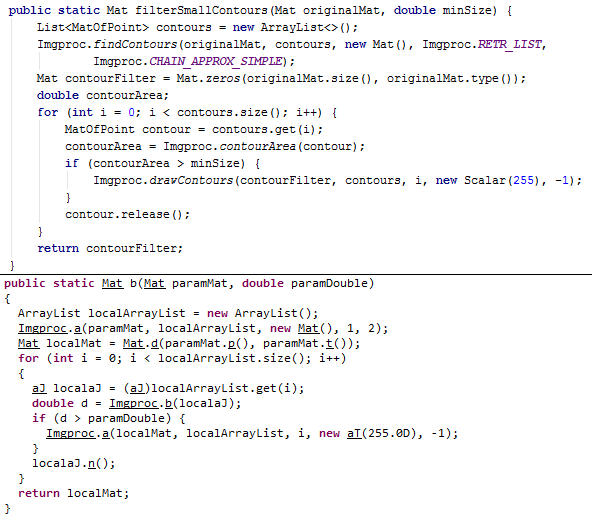
\includegraphics[scale=0.9]{app_obfus}
	\centering
	\caption{Horní část ukázky je zdrojový kód. Dolní je dekompilovaný obfuskovaný kód. \label{fig:app_obfus}}
\end{figure} 
\FloatBarrier

Jakmile je připravena JAR knihovna, spustí se plugin Launch4J, který vytvoří spouštěcí soubor pro platformu Windows. Je možné spouštět aplikaci i přes JAR, jelikož je odděleno od exe souboru, ale takto je to pohodlnější pro uživatele Windows. V exe souboru je také zakomponována kontrola minimální verze Javy.

\section{Modul Dev}
Modul Dev slouží pouze k vývoji algoritmů a není zahrnut do sestavení aplikace pro uživatele. Vznikl proto, že autor nemohl nalézt žádné vývojové nástroje pro Javu, které by byly kompatibilní s OpenCV a byly vhodné pro účel práce. Obsahuje pouze prosté \gls{glos:GUI}, které se z větší části generuje pomocí reflexe. Aby bylo možné pracovat s algoritmy v reálném čase a sledovat tak přímo, co který algoritmus s určitou konfigurací na konkrétním snímku dělá bylo nutné zasáhnout do logiky programu. Je snaha tento zásah řešit pouze v tomto modulu, ale některé nutné úpravy byly udělány i ve třídě Buffer (neomezená kapacita a nemažou se data) a VideoFrame(metody pro ukládání snímku algoritmu), fungují však pouze pokud je globálně zapnutý vývojový mód, a tak není ovlivněn běžný chod programu.

V rozhraní je stejně tak jako v aplikaci spuštěn MainController, který obsahuje jen volbu algoritmu a souboru, který má být zpracován, lze zpracovávat pouze jeden soubor a algoritmus najednou. Po spuštění programu je vystavěno vývojové rozhraní, které je vidět na obrázku \ref{fig:dev_debug}. Pomocí reflexe jsou získána všechna pole z třídy a ta, která obsahují anotaci @DevInterfaceField (ukázka na obrázku \ref{fig:core_new}), se zpracují a vytvoří se z nich ovládací prvek na základě hodnoty v atributu fieldType. Ovládací prvky mohou být: zaškrtávací políčko (pro booelan), posuvník (int, double, ...), obyčejné pole (string, int, ...) a výčtový typ. Výčtový typ je použit pro ukládání snímku algoritmu v daném kroku např. obrázek \ref{fig:dev_enum}.

\begin{figure}[h]
	
\includegraphics[scale=0.9]{dev_enum}
	\centering
	\caption{Ukázka konverze z BGR do HSV a následné uložení snímku pro vývoj. \label{fig:dev_enum}}
\end{figure} 
\FloatBarrier

\begin{figure}[h]
	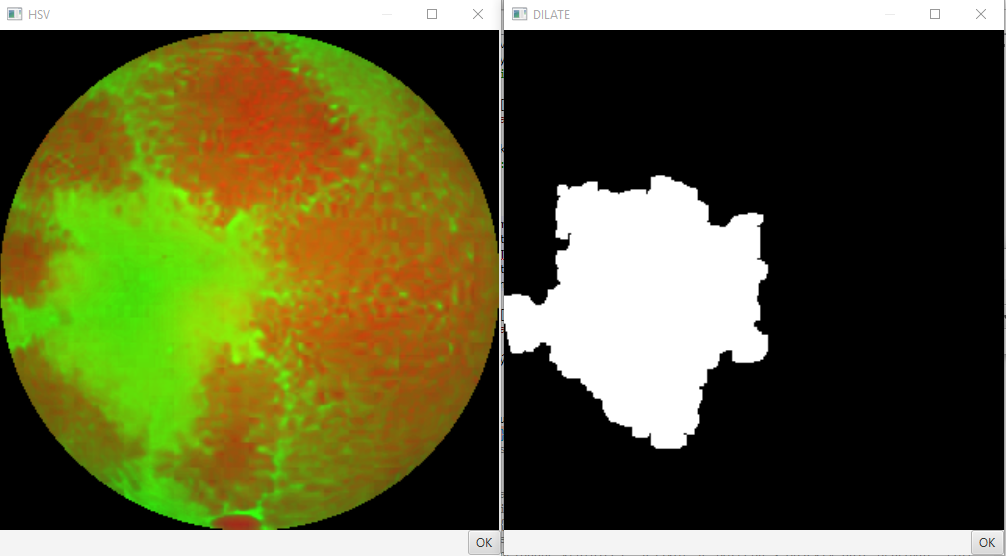
\includegraphics[scale=0.4]{dev_snap}
	\centering
	\caption{Ukázka snímků algoritmu. Vlevo převod do HSV, vpravo dilatace. \label{fig:dev_snap}}
\end{figure} 
\FloatBarrier

Pro běh programu je spuštěn AnalyzeTask z modulu Core pro získání a zpracování dat. K tomu je spuštěno další vlákno, kde běží BufferPlayer, který je potomkem AbstractBufferTask z modulu Core. Ten zpracovává data z Bufferu s aktuální konfigurací a také zobrazuje vybraná data snímků algoritmu v rozhraní, na obrázku \ref{fig:dev_snap} jsou vidět snímky z algoritmu. BufferPlayer také ukládá všechny detekované artefakty a k nim i snímky na disk pro rychlejší orientaci, co je detekováno. Jak je vidět na obrázku \ref{fig:dev_debug}, tak rozhraní disponuje ještě pauzou, posuvníkem rychlosti, opakováním a přechodem na konkrétní snímek v bufferu.



\begin{figure}[h]
	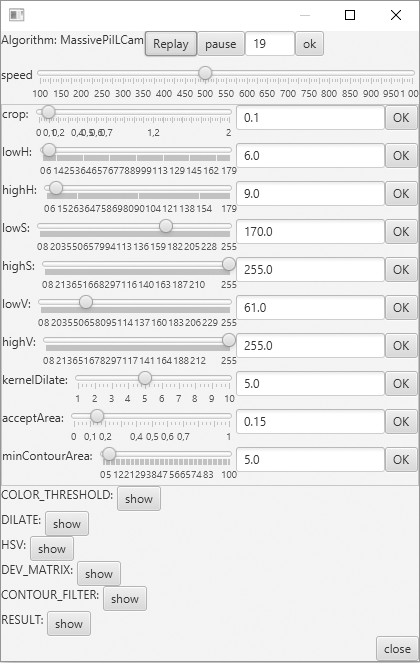
\includegraphics[scale=0.9]{dev_debug}
	\centering
	\caption{Vývojové rozhraní konkrétního algoritmu. \label{fig:dev_debug}}
\end{figure} 
\FloatBarrier


	\chapter{Testování vyvinutého řešení}
Testování a vývoj algoritmu byl prováděn především empiricky. K dispozici byl nejdříve malý vzorek dat, který byl dodán Fakultní nemocnicí Hradec Králové. Tento vzorek obsahoval 21 patologických videí, kde se vyskytovaly různé nemoci a 16 videí bez patologických výskytů. Každý snímek obsahoval 201 framů. Jelikož tato data byla extrahována za pomocí proprietárního softwaru dodávaného ke kamerám, tak kvalita dat nebyla nijak valná. U toho vzorku bylo lékaři označeno i, to co je na snímkách špatně.

Druhý vzorek dat byl získán od nemocnice až po vyvinutí algoritmů a softwaru. Měl tedy za úkol prokázat vyvinuté řešení na větším vzorku dat. U toho vzorku se však postrádá informace od profesionálů, jaká část obsahuje patologické nálezy a kvůli velkému množství dat to lze určit jen přibližně. Celkem se jedná o tři celé průchody kamerou, kde je patologický nález. Dva průchodu jsou z kamery PillCam celkem o 23608 framech a zbývající je z kamery od výrobce EndoCapsule o 87076 framech. Tento soubor dat je výrazně kvalitnější, jelikož ve spolupráci s akademií věd České republiky bylo použito jejich technologií pro extrakci dat z kamer. Na obrázku \ref{fig:vzorky} je vidět rozdíl v kvalitě obou vzorků.

\begin{figure}[h]
	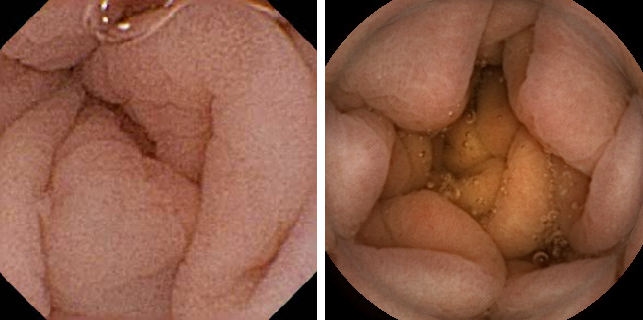
\includegraphics[scale=0.5]{vzorky}
	\centering
	\caption{Ukázka rozdílů kvality obou vzorků. Vlevo první vzorek, vpravo druhý vzorek \label{fig:vzorky}}
\end{figure} 

Vývoj a testování algoritmu detekce malých skvrn probíhal v různých etapách a od původního návrhu algoritmu do dnešní podoby se změnilo hodně věcí a byly použity jiné přístupy. Původní návrh byl nejdříve založen na adaptivním binárním práhování, ale to bylo zcela neúspěšné. Později byla snaha detekovat krvavé skvrny pomocí hranových detektorů konkrétně Cannyho detektor. To vedlo k lepšímu výsledku, nicméně chybovost byla příliš veliká a hrany se občas ztráceli vůči pozadí. Nakonec bylo zvoleno filtrování barev v HSV spektru, kde bylo dosaženo nejlepších výsledků a v kombinaci s hranovým detektorem pro odstranění míst bez hran se jeví jako optimální řešení. Testování později odhalilo, zejména v druhém vzorku dat, že druhý filtr barev pro zpřesnění výsledků není tak důležitý a jeho dopad v konečném výsledku není příliš markantní.

Druhý algoritmus byl značně přímočařejší a vzhledem k tomu, že autor již měl zkušenosti z prvního algoritmu, tak se spíše jednalo o nastavování správných hodnot v konfiguraci.

\section{Metodologie testování}
\label{sec:metodologie}
Pro měření úspěšnosti algoritmů jsou použity standardní postupy v počítačovém vidění pro určení efektivity algoritmu. Je tedy vypočítána hodnota \gls{glos:FRR} a \gls{glos:FAR} dle následujících vzorců.
\begin{equation*}
\gls{glos:FRR} = \frac{\gls{glos:FN}}{\gls{glos:TP}+\gls{glos:TN}+\gls{glos:FP}+\gls{glos:FN}} 
\end{equation*}
\begin{equation*}
\gls{glos:FAR} = \frac{\gls{glos:FP}}{\gls{glos:TP}+\gls{glos:TN}+\gls{glos:FP}+\gls{glos:FN}} 
\end{equation*}
V klinických testech se v lékařské komunitě používají hodnoty Senzitivita (\gls{glos:SE}) a Specificita (\gls{glos:SP})\cite{clinical}. Senzitivita je procentuální šance na detekci pacienta, který je nemocný a není tak špatně označen jako zdravý. Dalo by se říct, že opakem senzitivity je specificita. Při specificitě se jedná o správné detekování pacienta, který není nemocný a není špatně označen, jako pozitivní. Určuje se dle následujících vzorců.
\begin{equation*}
\gls{glos:SE} = \frac{\gls{glos:TP}}{\gls{glos:TP}+\gls{glos:FN}} 
\end{equation*}
\begin{equation*}
\gls{glos:SP} = \frac{\gls{glos:TN}}{\gls{glos:TN}+\gls{glos:FP}} 
\end{equation*}

V tabulce \ref{tab:vzorky} je vidět, kolik je skutečně pozitivních snímků v každém vzorku. Do tabulky jsou zahrnuty pouze ty vzorky, které obsahují krev. Ostatní vzorky buď obsahují jiné nemoci, nebo nejsou pozitivní. Každý vzorek také vždy neobsahuje krev, jež se dá snadno detekovat. Např. na vzorku z endocapsule je po cca 50\% vzorku masivní krvácení, kde se pak na každém snímku od vzniku problému vyskytuje alespoň slabá, místy růžová krev, která je již smíchána s jinými tekutinami, a tak nevyznačuje známky krve definované v algoritmu (dalo by se říct, že často je to spíše růžová voda). Počet snímků s krví u všech případů není úplně přesný, protože autor nemá k dispozici přesné počty, a tak musel vzorky projít ručně a provést odhad, který může být lehce nepřesný.

\begin{table}[h]
	\centering
	\begin{tabular}{|c|c|c|}
		\hline
		\bf Název souboru &  \bf Počet snímků & \bf Počet snímků s krví \\ \hline
		Endocapsule & 87076 & 45320 \\ \hline
		PillCam 1 & 13433 & 32 \\ \hline
		PillCam 2 & 10175 & 15 \\ \hline
		PAT07.avi & 201 & 5 \\ \hline
	\end{tabular}
	\caption{Jednotlivé vzorky s počtem krvavých snímků}
	\label{tab:vzorky}
\end{table}
\section{Výsledky testování}
Následující tabulka \ref{tab:vyslekdy_1} a \ref{tab:vyslekdy_2} ukazuje výsledky testování. Byly testovány všechny vzorky, vždy dle konfigurace pro ně určené. Pro jaký vzorek byla která konfigurace použita, je vidět v příloze \ref{sec:prilohaKonfig}. Ve výsledkových tabulkách jsou brány oba algoritmy jako jeden, a to z toho důvodu, že pro určení konečného výsledku je irelevantní, jestli to detekoval algoritmus A nebo B. Proto jsou vzaty výsledky obou algoritmů a je provedeno sjednocení. Také by bylo velmi problematické určit, co který algoritmus má detekovat a podle toho ho také hodnotit. Vybrané konkrétní výsledky algoritmů jsou vidět na obrázku \ref{fig:vysledy}. 
\begin{table}[h]
	\begin{adjustwidth}{-.5in}{-.5in} 
	\centering
	\begin{tabular}{|c|c|c|c|c|c|c|c|c|c|}
		\hline
		\bf Název souboru & \bf Detekováno & \bf \gls{glos:TP} & \bf \gls{glos:FP} & \bf \gls{glos:TN} & \bf \gls{glos:FN} & \bf \gls{glos:FRR} & \bf \gls{glos:FAR} & \bf \gls{glos:SE} & \bf \gls{glos:SP} \\ \hline
		PAT21.avi & 0 & 0 & 0 & 201 & 0 & 0,00\% & 0,00\% & N/A & 100,00\% \\ \hline
		PAT20.avi & 0 & 0 & 0 & 201 & 0 & 0,00\% & 0,00\% & N/A & 100,00\% \\ \hline
		PAT19.avi & 0 & 0 & 0 & 201 & 0 & 0,00\% & 0,00\% & N/A & 100,00\% \\ \hline
		PAT18.avi & 0 & 0 & 0 & 201 & 0 & 0,00\% & 0,00\% & N/A & 100,00\% \\ \hline
		PAT17.avi & 1 & 0 & 1 & 200 & 0 & 0,00\% & 0,50\% & N/A & 99,50\% \\ \hline
		PAT16.avi & 5 & 0 & 5 & 196 & 0 & 0,00\% & 2,49\% & N/A & 97,51\% \\ \hline
		PAT15.avi & 1 & 0 & 1 & 200 & 0 & 0,00\% & 0,50\% & N/A & 99,50\% \\ \hline
		PAT14.avi & 1 & 0 & 1 & 200 & 0 & 0,00\% & 0,50\% & N/A & 99,50\% \\ \hline
		PAT13.avi & 0 & 0 & 0 & 201 & 0 & 0,00\% & 0,00\% & N/A & 100,00\% \\ \hline
		PAT12.avi & 0 & 0 & 0 & 201 & 0 & 0,00\% & 0,00\% & N/A & 100,00\% \\ \hline
		PAT11.avi & 0 & 0 & 0 & 201 & 0 & 0,00\% & 0,00\% & N/A & 100,00\% \\ \hline
		PAT10.avi & 0 & 0 & 0 & 201 & 0 & 0,00\% & 0,00\% & N/A & 100,00\% \\ \hline
		PAT09.avi & 0 & 0 & 0 & 201 & 0 & 0,00\% & 0,00\% & N/A & 100,00\% \\ \hline
		PAT08.avi & 0 & 0 & 0 & 201 & 0 & 0,00\% & 0,00\% & N/A & 100,00\% \\ \hline
		PAT07.avi & 4 & 4 & 0 & 196 & 1 & 0,50\% & 0,00\% & 80,00\% & 100,00\% \\ \hline
		PAT06.avi & 0 & 0 & 0 & 201 & 0 & 0,00\% & 0,00\% & N/A & 100,00\% \\ \hline
		PAT05.avi & 0 & 0 & 0 & 201 & 0 & 0,00\% & 0,00\% & N/A & 100,00\% \\ \hline
		PAT04.avi & 0 & 0 & 0 & 201 & 0 & 0,00\% & 0,00\% & N/A & 100,00\% \\ \hline
		PAT03.avi & 0 & 0 & 0 & 201 & 0 & 0,00\% & 0,00\% & N/A & 100,00\% \\ \hline
		PAT02.avi & 3 & 0 & 3 & 198 & 0 & 0,00\% & 1,49\% & N/A & 98,51\% \\ \hline
		PAT01.avi & 0 & 0 & 0 & 201 & 0 & 0,00\% & 0,00\% & N/A & 100,00\% \\ \hline
		NOR9.avi & 0 & 0 & 0 & 201 & 0 & 0,00\% & 0,00\% & N/A & 100,00\% \\ \hline
		NOR8.avi & 0 & 0 & 0 & 201 & 0 & 0,00\% & 0,00\% & N/A & 100,00\% \\ \hline
		NOR7.avi & 2 & 0 & 2 & 199 & 0 & 0,00\% & 1,00\% & N/A & 99,00\% \\ \hline
		NOR6.avi & 0 & 0 & 0 & 201 & 0 & 0,00\% & 0,00\% & N/A & 100,00\% \\ \hline
		NOR5.avi & 0 & 0 & 0 & 201 & 0 & 0,00\% & 0,00\% & N/A & 100,00\% \\ \hline
		NOR4.avi & 0 & 0 & 0 & 201 & 0 & 0,00\% & 0,00\% & N/A & 100,00\% \\ \hline
		NOR3.avi & 0 & 0 & 0 & 201 & 0 & 0,00\% & 0,00\% & N/A & 100,00\% \\ \hline
		NOR2.avi & 0 & 0 & 0 & 201 & 0 & 0,00\% & 0,00\% & N/A & 100,00\% \\ \hline
		NOR16.avi & 0 & 0 & 0 & 201 & 0 & 0,00\% & 0,00\% & N/A & 100,00\% \\ \hline
		NOR15.avi & 0 & 0 & 0 & 201 & 0 & 0,00\% & 0,00\% & N/A & 100,00\% \\ \hline
		NOR14.avi & 0 & 0 & 0 & 201 & 0 & 0,00\% & 0,00\% & N/A & 100,00\% \\ \hline
		NOR13.avi & 0 & 0 & 0 & 201 & 0 & 0,00\% & 0,00\% & N/A & 100,00\% \\ \hline
		NOR12.avi & 0 & 0 & 0 & 201 & 0 & 0,00\% & 0,00\% & N/A & 100,00\% \\ \hline
		NOR11.avi & 0 & 0 & 0 & 201 & 0 & 0,00\% & 0,00\% & N/A & 100,00\% \\ \hline
		NOR10.avi & 0 & 0 & 0 & 201 & 0 & 0,00\% & 0,00\% & N/A & 100,00\% \\ \hline
		NOR1.avi & 47 & 0 & 47 & 154 & 0 & 0,00\% & 23,38\% & N/A & 76,62\% \\ \hline
	\end{tabular}
	\caption{Výsledky testování prvního vzorku}
	\label{tab:vyslekdy_1}
	\end{adjustwidth}
\end{table}

\begin{table}[h]
	\begin{adjustwidth}{-.5in}{-.5in} 
		\centering
		\begin{tabular}{|c|c|c|c|c|c|c|c|c|c|}
			\hline
				\bf Název souboru & \bf Detekováno & \bf \gls{glos:TP} & \bf \gls{glos:FP} & \bf \gls{glos:TN} & \bf \gls{glos:FN} & \bf \gls{glos:FRR} & \bf \gls{glos:FAR} & \bf \gls{glos:SE} & \bf \gls{glos:SP} \\ \hline
			Endocapsule & 37889 & 35546 & 2343 & 39413 & 9774 & 11,22\% & 2,69\% & 78,43\% & 94,39\% \\ \hline
			PillCam 1 & 159 & 24 & 135 & 13266 & 8 & 0,06\% & 1,00\% & 75,00\% & 98,99\% \\ \hline
			PillCam 2 & 79 & 12 & 67 & 10093 & 3 & 0,03\% & 0,66\% & 80,00\% & 99,34\% \\ \hline
		\end{tabular}
		\caption{Výsledky testování druhého vzorku}
		\label{tab:vyslekdy_2}
	\end{adjustwidth}
\end{table}

\begin{figure}[h]
	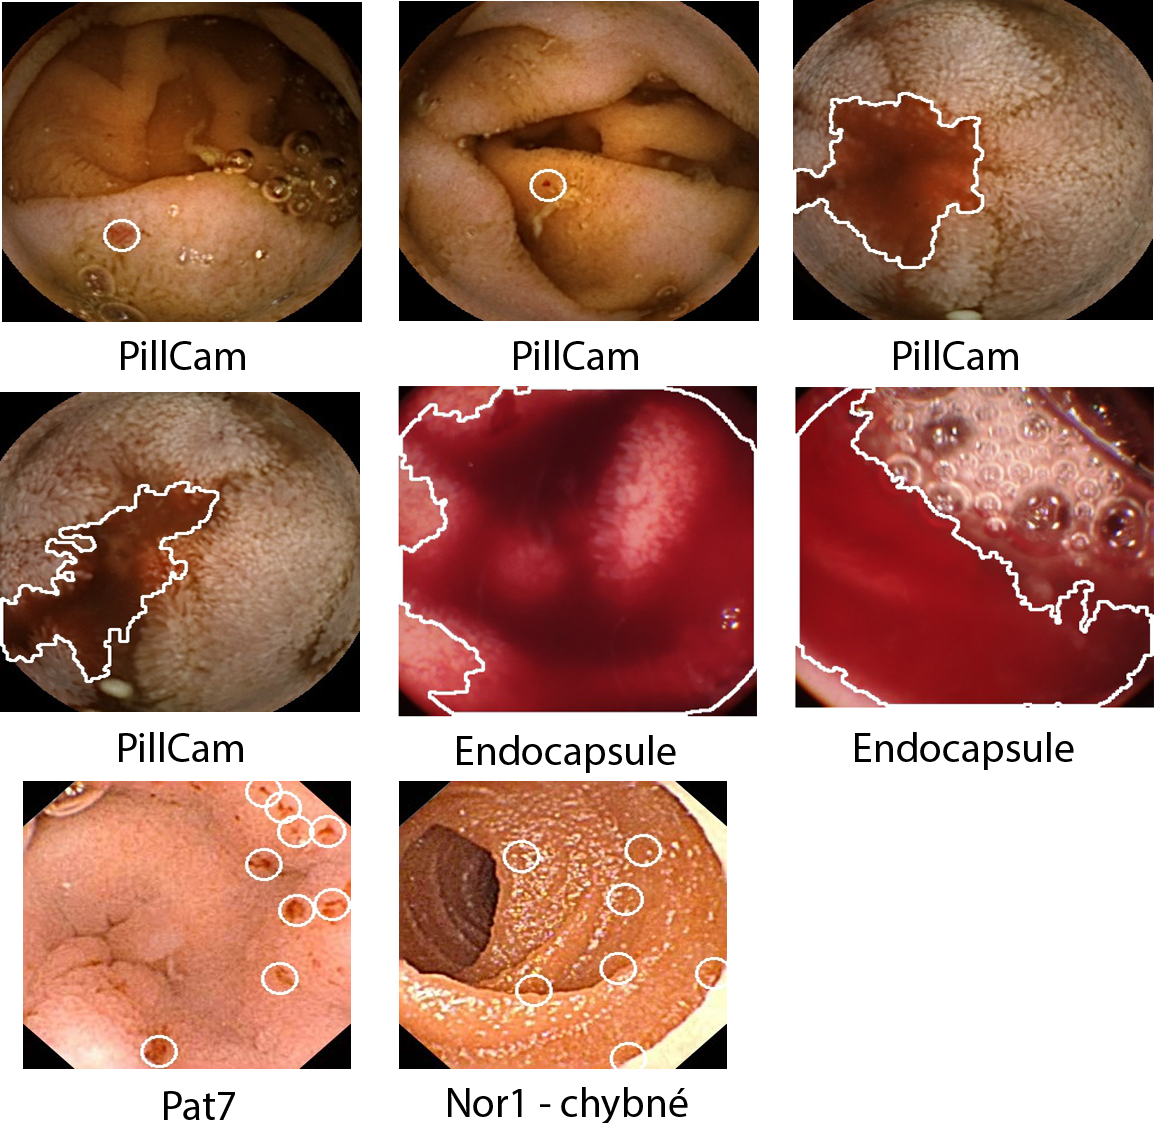
\includegraphics[scale=1.6]{result}
	\centering
	\caption{Ukázka vybraných výsledků \label{fig:vysledy}}
\end{figure}

\section{Zhodnocení testování}
Testování algoritmů probíhalo ve dvou etapách. V první etapě se algoritmy vyvíjeli a testovali na prvním vzorku dat. Kde se dle tabulky \ref{tab:vyslekdy_1} dosáhlo uspokojivých výsledků.

V druhé etapě byl obdržen druhý vzorek dat z reálných pacientů. Po aplikaci konfigurace z prvního vzorku a spuštění testů nad druhým došlo k téměř absolutnímu neúspěchu. Aplikace nebyla schopna detekovat ani výrazné krvácení. Bylo zapotřebí vytvořit konfiguraci, zejména na filtr dle barev, pro každý vzorek zvlášť. Stejné chování je zaznamenáno i mezi odlišnými výrobci kamer v druhém vzorku, každá kamera má odlišné barevné spektrum, které dokáže snímat a tak není možné použít univerzální řešení pro všechno. Výsledky testování druhého vzorku jsou vidět v tabulce \ref{tab:vyslekdy_2}.

Při testování jinak nedošlo ke změnám algoritmů či programu. Vše fungovalo, tak jak bylo očekáváno. Pouze se vytvořili nové konfigurace pro algoritmy. Porovnání nové metody o proti metodám zmíněných ve vědeckých článcích nebylo možné, protože není k dispozici stejný datový vzorek. V následující kapitole budou detailněji rozebrány a zhodnoceny samotné výsledky.
	\chapter{Diskuze nad výsledky}
Z tabulky \ref{tab:avgres} je vidět, že průměrná senzitivita u pozitivních videí je 78.36\%. To se může zdát jako málo, ale vzhledem k tomu, že se krev nachází ve střevech v různé podobě a tvarech, tak nelze vždy určit krev všechnu, jelikož je to mnohdy velmi obtížné. Co je důležité, že ve všech případech byl určen zdroj krvácení, případně jeho největší části. Ostatní nedetekované objekty pak mohou být např. smíchaná krev s tekutinami nebo její velmi malé částečky po okrajích snímku mnohdy již dříve detekované anomálie na snímcích předchozích. Pro relevantnost testů je však nutné tyto objekty zahrnout do \gls{glos:FN}, jelikož odborníci jsou schopni je určit za pomocí jejich predikce a zkušeností. Také pro vyšetření pacienta je podstatné vědět, kde se nachází zdroj krvácení nebo jeho velká část.

\begin{table}[h]
	\centering
	\begin{tabular}{|c|c|c|c|c|}
		\hline
		\bf Název &  \bf \gls{glos:FRR} & \bf \gls{glos:FAR} & \bf \gls{glos:SE} & \bf \gls{glos:SP} \\ \hline
		Pozitivní videa & 2,95\% & 1,09\% & 78,36\% & 98,18\% \\ \hline
		Negativní videa & 0,00\% & 0,83\% & N/A & 99,17\% \\ \hline
	\end{tabular}
	\caption{Průměrné výsledky}
	\label{tab:avgres}
\end{table}

Specificita a \gls{glos:FAR} u všech videí je, až na jednu výjimku, velice dobrá a je tak možné rychle určit, zda-li pacient je zdráv či nikoliv. Výjimkou je video NOR1.avi, kde bylo rozeznáno 23.28\% mylně pozitivních snímků viz. tabulka \ref{tab:vyslekdy_1}. To je způsobeno tím, že se ve videu nachází hodně odlesků, které pak vytvářejí malé anomálie.

Hodnota \gls{glos:FRR} se drží v přijatelných mezích a nejsou příliš odmítány i snímky, které obsahují krev. Výjimkou je vzorek Endocapsule a to z důvodu, že se zde nachází masivní krvácení, a jak již bylo zmíněno výše, tak některé snímky již nelze přesněji určit a je podstatné, že se našel zdroj krvácení. Pravděpodobně by nevznikly z něčeho, co se nepodařilo určit, a test by tak závisel na tom, jestli se poznají vedlejší efekty krvácení.

Ohledně výsledků toho, jak si na tom stojí software, tak během testování byly zjištěny technické nedostatky a to zejména v ukládání dočasných výsledků algoritmu pro pozdější generování výstupních souborů. Při testování vzorku z Endocapsule, kde bylo detekováno 37889 objektů, tak byly nároky na paměť enormní a musel se testovaný vzorek rozdělit na více částí. Také občas působila problémy knihovna OpenCV. Jelikož se jedná o nativní přístup, tak zde byl problém s garbage collectorem, který neodstraňuje nativní objekty, a proto se muselo dávat pozor, aby se všechny vytvořené nativní objekty korektně zrušily za pomocí k tomu určených funkcí v OpenCV. Jinak výkonnost a optimalizace algoritmů je uspokojivá. Například oba vzorky z PillCam trvalo zpracovat dvě minuty a šestnáct vteřin na průměrném PC.

Naplnění funkčních a nefunkčních požadavků na software se podařilo naplnit s dvěma nedostatky. Z výsledků testování vyplynula nedostatečná optimalizaci při držení detekovaných hodnot a tím velké nároky na paměť. A software umí načítat nativní OpenCV knihovny pouze pro MS Windows. Pro ostatní OS, které OpenCV podporuje není hotové načítání knihoven z důvodu absence těchto prostředí při vývoji.
\section{Možný směr budoucího vývoje}
Budoucí vývoj by se mohl ubírat opravnou technických částí softwaru čí jeho vylepšením, na které už nebyl vzhledem časové náročnosti čas. V bodech by se jednalo hlavně o tyto záležitosti:
\begin{itemize}
	\item Implementace MapDB pro vyřešení paměťové náročnosti při velkých datech nebo zaměnit způsob ukládání výsledků algoritmu, např. pouze jako číslo snímku, nikoliv celý snímek, a zpětně je pak dohledávat.
	\item Dodělat načítání nativních OpenCV knihoven pro ostatní OS.
	\item Implementace Spring Boot a nahrazení frameworku Weld, který musel být odstraněn.
	\item Větší škálování vláken pro algoritmy a čtení více dat z bufferu jedním algoritmem. Momentálně se snímky z bufferu zpracovávají jeden po jednom.
	\item Neanalyzovat již pozitivní snímek určený jiným algoritmem.
	\item Nastavení neměnných konstant algoritmu při prvním běhu a nepočítat je vždy znova pro každý snímek. Toto platí pouze za předpokladu, že všechny snímky budou ve vzorku stejné. 
	\item Rozložit některé části algoritmu na více vláken a zpracovávat asynchronně části na sobě nezávislé.
	\item Implementovat webové rozhraní. Uživatel by přistupoval k programu pouze na bázi tenkého klienta a všechny operace by se děly na straně serveru. To by mohlo přinést rychlejší zpracování a případně prohlížení výsledků i na mobilních zařízení/tabletech.
\end{itemize}

Dále by bylo nutné otestovat software na ještě větším množství dat a případně podle toho doladit algoritmy. Co se týče algoritmů, tak z detekce malých skvrn by šla odstranit část pro zpřesnění výsledků, jelikož se ukázalo, že není tak důležitá. Nejdůležitějším bodem budoucího vývoje zůstává rozšíření programu o další algoritmy na jiné nemoci a vyzkoušení dalších technik, např. neuronové sítě pro detekci nových věcí.
	\chapter{Závěr}
Cílem práce bylo analyzovat možnosti počítačového vidění v biomedicíně. Byla představena kapslová endoskopie, její využití a možnosti. Dále se práce zabývala představením počítačového vidění a jeho základními principy. Průzkum aktuálního stavu trhu sumarizoval již hotové řešení od výrobců kapslí, to bohužel vzhledem k uzavřenosti programů nepřineslo mnoho výsledků.

Praktická část se zabývala vývojem nového softwaru, který by byl alespoň částečně konkurence schopný a uměl detekovat krev, případně v budoucnu i další choroby. Vzorky pro testování byly dodány Fakultní nemocnicí Hradec Králové. 

Samotný vývoj software se ukázal jako časově náročný, ale obešel se bez výraznějších problémů, jelikož zvolené technologie byly autorovi dobře známé. S algoritmy byla daleko větší práce. Autor měl sice předchozí zkušenosti s počítačovým viděním, ale nebyly nikterak četné. Neocenitelnou pomoc pro vývoj algoritmů skýtaly konzultace s Dr. Orcanem Alparem.

Testování ukázalo, že software je schopný detekovat krev ve střevech s vysokou přesností. Aby byly výsledky průraznější, bylo by vhodné v tomto projektu pokračovat i mimo tuto diplomovou práci a provést další, rozsáhlejší testy. Zatím je vývoj projektu na dobré cestě a myslím si, že výsledky jsou uspokojivé.
	\begin{flushleft}
\printbibliography[heading=bibintoc,title={Literatura}]
\end{flushleft}
\cleardoublepage{}

\newglossaryentry{glos:GUI}{name=GUI, description={Graphical user interface - uživatelské rozhraní}}
\newglossaryentry{glos:CV}{name=CV, description={Computer vision - počítačové vidění}}
\newglossaryentry{glos:EER}{name=EER, description={Equal error rate - přijatelná míra chyb}}
\newglossaryentry{glos:FAR}{name=FAR, description={False acceptance rate - míra špatně detekovaných objektů}}
\newglossaryentry{glos:FRR}{name=FRR, description={False rejection rate - míra chybně odmítnutých objektů}}
\newglossaryentry{glos:AVI}{name=AVI, description={Multimediální video formát}}
\newglossaryentry{glos:JPG}{name=JPG, description={Metoda komprese obrázku}}
\newglossaryentry{glos:JNA}{name=JNA, description={Java native access - funkcionalita pro volání nativních knihoven z Javy}}
\newglossaryentry{glos:CDI}{name=CDI, description={Contexts and Dependency Injection - standart pro vkládání závislostí a kontextu. Poprvé byl uveřejněn pro Javu EE 6}}
\newglossaryentry{glos:MVC}{name=MVC, description={Model-View-Controller - návrhový vzor}}
\newglossaryentry{glos:WCE}{name=WCE, description={Wireless capsule endoskopy - bezdrátová kapslová endoskopie}}
\newglossaryentry{glos:TP}{name=TP, description={True positivity - pozitivní anomálie}}
\newglossaryentry{glos:FP}{name=FP, description={False positivity - falešně pozitivní anomálie}}
\newglossaryentry{glos:TN}{name=TN, description={True negativity - nepozitivní anomálie}}
\newglossaryentry{glos:FN}{name=FN, description={False negativity - falešně nepozitivní anomálie}}
\newglossaryentry{glos:MDR}{name=MDR, description={Missed detection rate - stejné jako FRR}}
\newglossaryentry{glos:SE}{name=SE, description={Sensitivity - pravděpodobnost detekce}}
\newglossaryentry{glos:SP}{name=SP, description={Specificity - přesnost detekce}}
\newglossaryentry{glos:ROI}{name=ROI, description={Rectangle of interest - čtverec/oblast zájmu}}
{\setstretch{1.0}
	\printglossary[nonumberlist]
}


\appendix
\pagenumbering{Roman}\addcontentsline{toc}{part}{Přílohy}\thispagestyle{empty}  \renewcommand{\appendixname}{P\v{r}iloha}%%přílohy, číslování římskými

\part*{Přílohy} %% rename

\listoffigures

\listoftables

\chapter{Konfigurace algoritmů}
\label{sec:prilohaKonfig}
V této příloze je konfigurace algoritmů a její vysvětlení.
\begin{table}[h]
	\begin{adjustwidth}{-.5in}{-.5in} 
		\centering
		\begin{tabular}{|l|l|c|c|}
			\hline
			\multicolumn{1}{|c|}{\bf Konfigurace} & \multicolumn{1}{c|}{\bf Význam} & \bf Málé skvrny & \bf Velké skvrny \\ \hline
			highH & \begin{tabular}[c]{@{}l@{}}maximální hranice filtru pro H kanál\\ ve formátu HSV\end{tabular} & Y & Y \\ \hline
			lowH & \begin{tabular}[c]{@{}l@{}}minimální hranice filtru pro H kanál\\ ve formátu HSV\end{tabular} & Y & Y \\ \hline
			highS & \begin{tabular}[c]{@{}l@{}}maximální hranice filtru pro S kanál\\ ve formátu HSV\end{tabular} & Y & Y \\ \hline
			lowS & \begin{tabular}[c]{@{}l@{}}minimální hranice filtru pro S kanál\\ ve formátu HSV\end{tabular} & Y & Y \\ \hline
			highV & \begin{tabular}[c]{@{}l@{}}maximální hranice filtru pro V kanál\\ ve formátu HSV\end{tabular} & Y & Y \\ \hline
			lowV & \begin{tabular}[c]{@{}l@{}}minimální hranice filtru pro V kanál\\ ve formátu HSV\end{tabular} & Y & Y \\ \hline
			kernelDilate & velikost jádra pro dilataci & Y & Y \\ \hline
			minContourArea & minimální velikost spojité oblasti & Y & Y \\ \hline
			highHPost & \begin{tabular}[c]{@{}l@{}}maximální hranice zpřesňujícího filtru\\ pro H kanál ve formátu HSV\end{tabular} & Y & N \\ \hline
			lowHPost & \begin{tabular}[c]{@{}l@{}}minimální hranice filtru zpřesňujícího filtru\\ pro H kanál ve formátu HSV\end{tabular} & Y & N \\ \hline
			highSPost & \begin{tabular}[c]{@{}l@{}}maximální hranice zpřesňujícího filtru\\ pro S kanál ve formátu HSV\end{tabular} & Y & N \\ \hline
			lowSPost & \begin{tabular}[c]{@{}l@{}}minimální hranice filtru zpřesňujícího\\ pro S kanál ve formátu HSV\end{tabular} & Y & N \\ \hline
			highVPost & \begin{tabular}[c]{@{}l@{}}maximální hranice zpřesňujícího filtru\\ pro V kanál ve formátu HSV\end{tabular} & Y & N \\ \hline
			lowVPost & \begin{tabular}[c]{@{}l@{}}minimální hranice filtru zpřesňujícího filtru\\ pro V kanál ve formátu HSV\end{tabular} & Y & N \\ \hline
			blurKernelSize & velikost jádra pro rozmazání & Y & N \\ \hline
			cannyThreshMin & minimálníh hranice práhování pro canny & Y & N \\ \hline
			cannyThreshMax & maximální hranice práhování pro canny & Y & N \\ \hline
			apertureSize & velikost sobelova operátoru & Y & N \\ \hline
			maxCircleRadius & maximální velikost kružnice & Y & N \\ \hline
			crop & hodnota oříznutí & Y & Y \\ \hline
			acceptArea & minimální procentuální velikost & N & Y \\ \hline
		\end{tabular}
		\caption{Konfigurace algoritmů}
		\label{tab:cfg}
	\end{adjustwidth}
\end{table}

\chapter{Konkrétní konfigurace algoritmů}
\label{sec:prilohaHodnoty}
V této příloze jsou konkrétní hodnoty konfigurace algoritmů, se kterou byli testovány data. Konfigurace jsou pouze jako textový výstup, jelikož konfigurační XML soubory jsou příliš velké.

\noindent
\begin{flushleft}
\textbf{Detekce malých skvrn - první vzorek\\}
apertureSize-3;
cannyThreshMax-175;
lowSPost-195;
blurKernelSize-3;
lowH-8;
lowVPost-200;
lowHPost-8;
highSPost-255;
highH-10;
lowS-190;
lowV-167;
highVPost-210;
minContourArea-5;
cannyThreshMin-140;
highHPost-9;
maxCircleRadius-15;
kernelDilate-10;
highS-255;
highV-220;
crop-0.1;
---\\
\textbf{Detekce malých skvrn - Endocapsule\\}
apertureSize-3;
cannyThreshMax-145;
lowSPost-135;
blurKernelSize-3;
lowH-165;
lowVPost-75;
lowHPost-165;
highSPost-255;
highH-179;
lowS-135;
lowV-75;
highVPost-191;
minContourArea-5;
cannyThreshMin-130;
highHPost-179;
maxCircleRadius-15;
kernelDilate-10;
highS-255;
highV-191;
crop-0.1;
---\\
\textbf{Detekce malých skvrn - PillCam\\}
apertureSize-3;
cannyThreshMax-145;
lowSPost-190;
blurKernelSize-3;
lowH-8;
lowVPost-160;
lowHPost-8;
highSPost-255;
highH-11;
lowS-190;
lowV-150;
highVPost-220;
minContourArea-5;
cannyThreshMin-130;
highHPost-11;
maxCircleRadius-15;
kernelDilate-10;
highS-255;
highV-220;
crop-0.1;
---\\
\textbf{Detekce velkých skvrn - první vzorek\\}
lowV-167;
acceptArea-0.15;
minContourArea-5;
lowH-8;
kernelDilate-5;
highS-255;
highH-10;
lowS-190;
crop-0.1;
highV-220;
---\\
\textbf{Detekce velkých skvrn - Endocapsule\\}
lowV-75;
acceptArea-0.15;
minContourArea-5;
lowH-165;
kernelDilate-5;
highS-255;
highH-179;
lowS-135;
crop-0.1;
highV-191;
---\\
\textbf{Detekce velkých skvrn - PilLCam\\}
lowV-61;
acceptArea-0.15;
minContourArea-5;
lowH-6;
kernelDilate-5;
highS-255;
highH-9;
lowS-170;
crop-0.1;
highV-255;
\end{flushleft}
	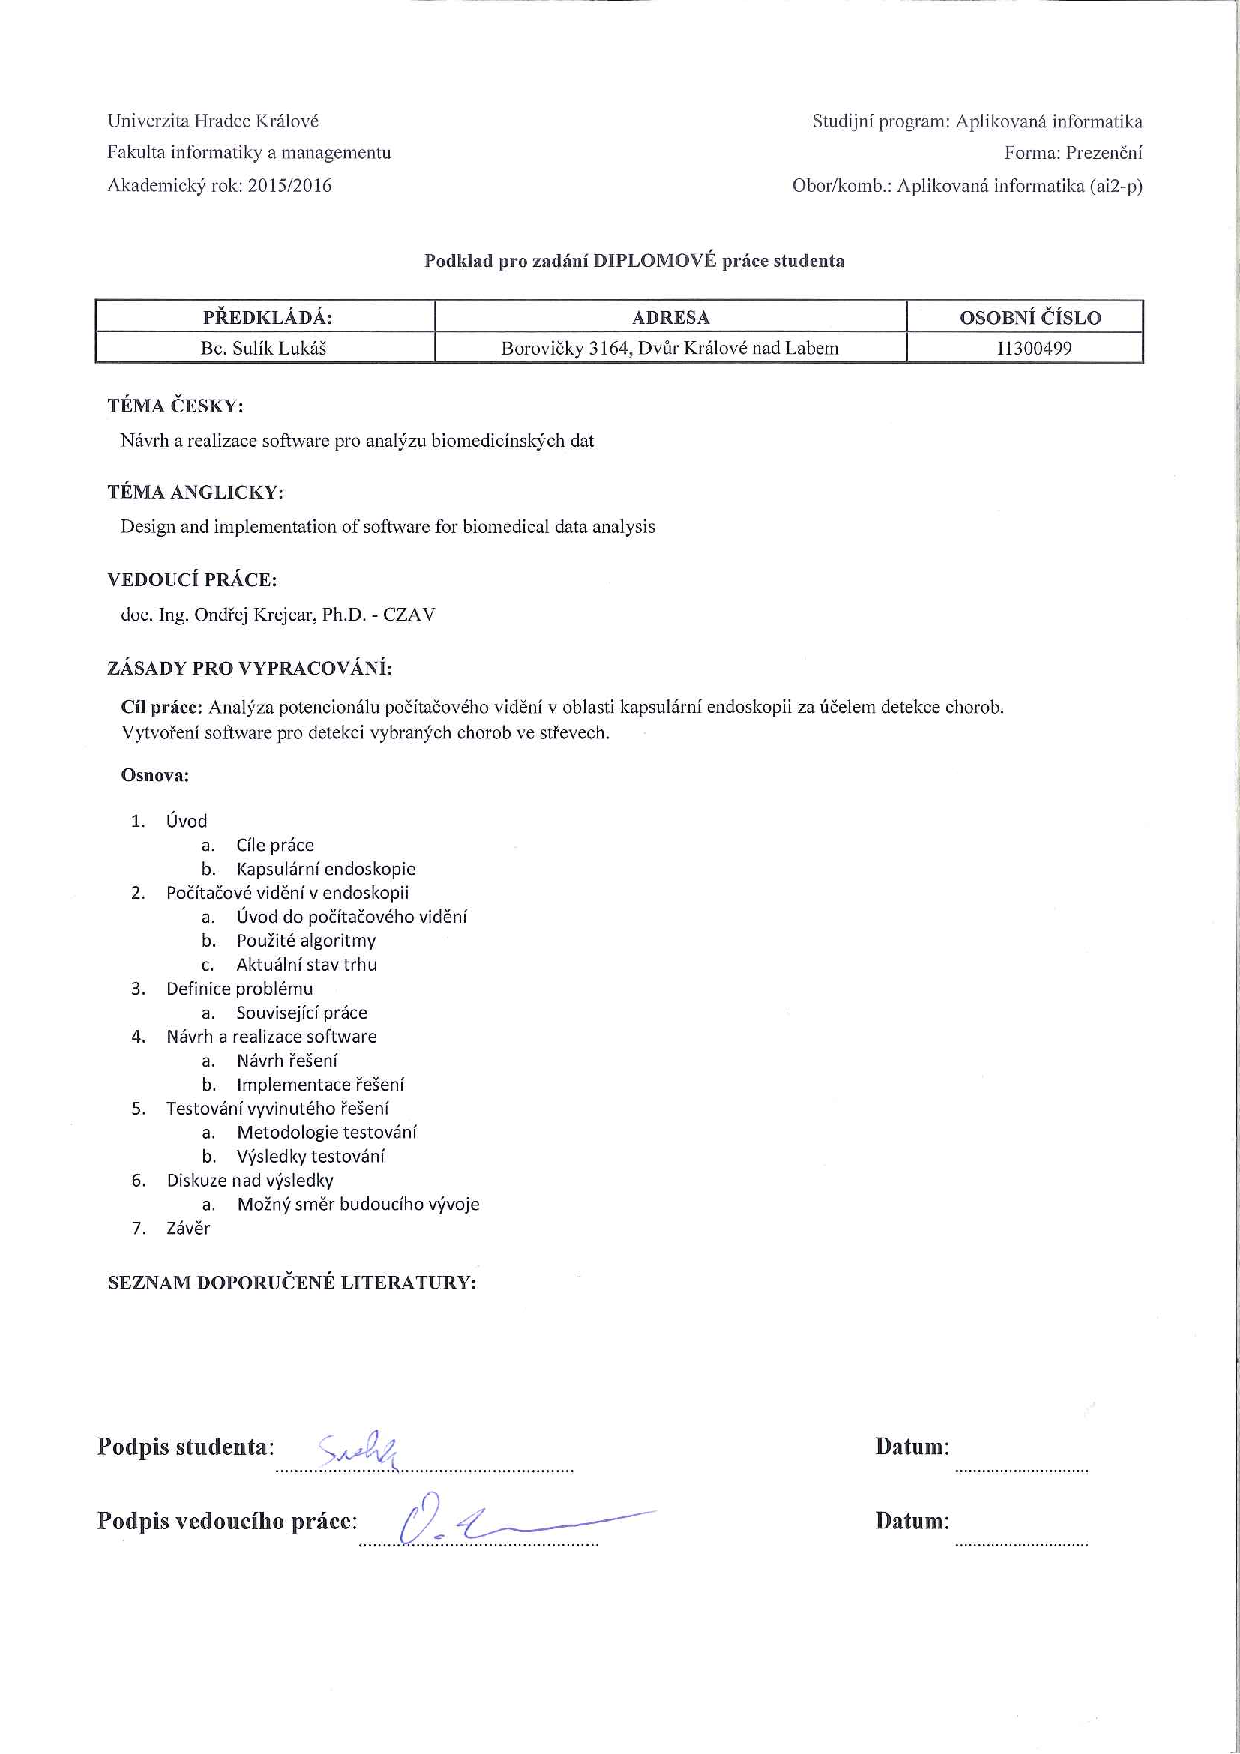
\includepdf[pages={1}]{zadani.pdf}
	
\end{document}
